\documentclass[11pt,oneside]{book}
\usepackage[margin=1in]{geometry}
\usepackage{amsmath,amssymb,amsthm}
\usepackage{graphicx,float,booktabs,xcolor,hyperref}
\usepackage{caption,subcaption}
% enumitem disabled
\usepackage{textcomp}
% tcolorbox disabled
\graphicspath{{figs/}}
\hypersetup{colorlinks=true, linkcolor=blue, citecolor=blue, urlcolor=blue}

\theoremstyle{definition}
\newtheorem{definition}{Definition}[chapter]
\newtheorem{proposition}[definition]{Proposition}
\newtheorem{theorem}[definition]{Theorem}
\newtheorem{lemma}[definition]{Lemma}
\newtheorem{remark}[definition]{Remark}
\newtheorem{example}[definition]{Example}

\title{\Huge\textbf{MIZN}\\
\Large A modular spectral solver for the K=3\\
noiseless CRRA rational-expectations equilibrium\\[1em]
\large Economic model, mathematical formulation,\\
Chebyshev discretization, and numerical algorithm}
\author{Companion volume to MIZN repository}
\date{}

\begin{document}
\frontmatter
\maketitle
\tableofcontents
\listoffigures

\chapter*{Preface}

This book is the definitive technical companion to the MIZN codebase: an end-to-end
treatment of the noiseless K=3 CRRA rational-expectations equilibrium (REE) problem,
from economic foundations through to a working numerical algorithm based on
symmetric Chebyshev spectral methods.

It is structured in seven parts:

\begin{description}
\item[Part I --- Economic setup.] The model, its primitives (agents, signals,
asset), the information structure, individual demands, and the market-clearing
problem. The 5-step Hellwig cycle as the natural fixed-point loop.

\item[Part II --- Mathematical formulation.] The exact equation system. The
price as a function $P(u_1,u_2,u_3)$. Boundary conditions and asymptotic limits.
Symmetries (S$_3$ and Z$_2$). The relationship to known closed-form cases
(CARA Hellwig 1980, fully revealing limit).

\item[Part III --- Chebyshev discretization.] Coordinate transformations, the
tensor Chebyshev basis, boundary conditions in Chebyshev, S$_3 \times$ Z$_2$
symmetric basis, per-agent evaluation via permutation, companion-matrix
contour root-find, Gauss-Legendre quadrature.

\item[Part IV --- Numerical algorithm.] The full pipeline from $P$ to $\Phi(P)$,
slice-evidence computation, Bayesian update, CRRA clearing, dense Newton
iteration, $\gamma$-continuation strategies.

\item[Part V --- Implementation in MIZN.] The module structure, build order,
testing strategy, the per-run execution-log system with auto-generated LaTeX
PDF reports.

\item[Part VI --- Validation.] CARA Hellwig closed-form gold test, symmetry
checks, spectral-decay diagnostics, $\gamma$-sweep reproduction of prior
machine-precision results.

\item[Part VII --- Outlook.] Past the $\gamma$-fold via pseudo-arclength
continuation; higher K extensions; the relationship to other REE models.
\end{description}

The text assumes graduate-level familiarity with Bayesian asset pricing and
basic numerical linear algebra (Newton's method, Chebyshev polynomials), but
attempts to develop every nontrivial step in full so that a careful reader
can implement MIZN from scratch using this document as the specification.

\mainmatter

\part{Economic Setup}
\label{part:econ}

\chapter{The Model: Primitives and Information Structure}

\section{What problem are we solving?}

A canonical question in financial economics is whether --- and how completely
--- equilibrium asset prices aggregate the dispersed private information of
many traders. In a \emph{fully revealing} equilibrium (FR), the price is a
sufficient statistic for the joint information of all agents: an outsider
observing only $P$ knows as much about the asset value as the union of all
agents' signals. In a \emph{partially revealing} equilibrium (PR), the price
reveals only some --- typically the projection along one linear combination of
signals --- leaving residual uncertainty even to a fully-Bayesian outside
observer.

Whether REE is FR or PR depends on the joint structure of preferences, signal
distributions, and the asset payoff. Two seminal results frame the
landscape:

\begin{itemize}
\item \textbf{Hellwig (1980).} In a Gaussian-signal Gaussian-supply-noise
linear REE with CARA agents, the equilibrium is partially revealing because
supply noise injects uncertainty into the price even when agents know the
signal distribution. Hellwig derived the linear coefficients in closed form;
this serves as our gold test (Chapter \ref{ch:hellwig_form}).

\item \textbf{Grossman \& Stiglitz (1980); paradox of informationally
efficient markets.} If REE is FR, no one has an incentive to gather information.
Equilibrium markets cannot be too informationally efficient.
\end{itemize}

The MIZN project tackles a less-studied variant: \textbf{noiseless K=3
CRRA REE with a binary asset value $v \in \{0,1\}$}. Removing supply noise
removes Hellwig's smoking gun for PR; replacing CARA with CRRA + a binary
asset introduces a Jensen-gap mechanism (concavity of demand in beliefs)
that \emph{may} generate PR for sufficiently low risk aversion $\gamma$.
Whether this PR equilibrium genuinely exists --- and what its properties are ---
is the substantive question, and answering it numerically requires a robust
fixed-point solver. That is MIZN.

\section{Primitives}

\subsection{The asset}

A single risky asset has uncertain payoff
\begin{equation}
v \in \{0, 1\}, \qquad \Pr(v=0) = \Pr(v=1) = \tfrac12.
\label{eq:asset}
\end{equation}
The binary structure simplifies Bayesian arithmetic: each posterior is a
single number $\mu \in [0,1]$ representing $\Pr(v=1 \mid \text{info})$.

\subsection{The agents and their signals}

There are $K=3$ symmetric agents indexed by $k \in \{1, 2, 3\}$. Each agent
$k$ observes a private noisy signal:
\begin{equation}
$u_k$ = v + \varepsilon_k, \qquad \varepsilon_k \sim \mathcal{N}\!\bigl(0,
\tau^{-1}\bigr),
\label{eq:signal}
\end{equation}
with the noises $\varepsilon_k$ mutually independent given $v$. The
\emph{signal precision} $\tau$ is a model parameter; in our worked example
we take $\tau = 2$.

Conditional on $v$, the signal $$u_k$$ is Gaussian with mean $v$ and variance
$1/\tau$. Writing the conditional density as $f_v$:
\begin{equation}
f_v(u) = \sqrt{\frac{\tau}{2\pi}}\,\exp\!\Bigl(-\tfrac{\tau}{2}(u - m_v)^2\Bigr),
\qquad m_0 = -\tfrac12,\ m_1 = +\tfrac12.
\label{eq:density}
\end{equation}

(Note: the convention $m_0 = -1/2$, $m_1 = +1/2$ rather than $m_0 = 0$,
$m_1 = 1$ is a centered re-parametrization; the relevant economics --- the
difference $m_1 - m_0 = 1$ and the precision $\tau$ --- is unchanged.)

\begin{figure}[H]
\centering
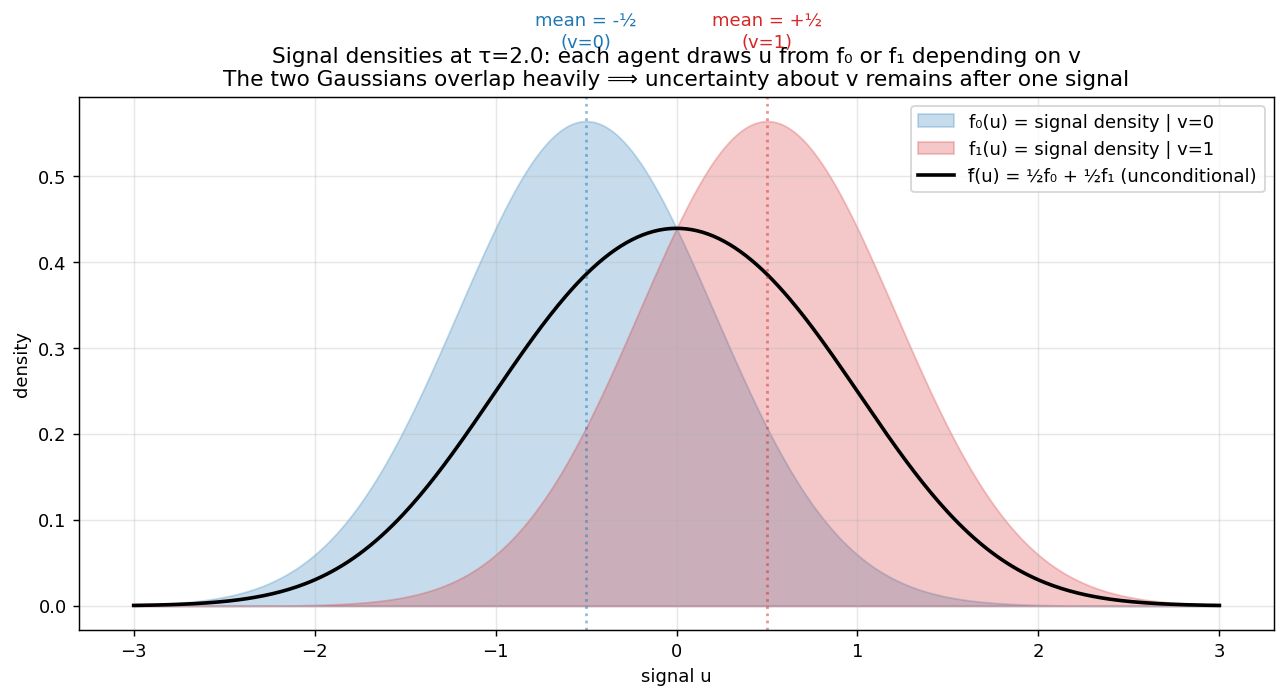
\includegraphics[width=0.85\linewidth]{15_signal_density.png}
\caption{The two conditional signal densities $f_0$ (blue) and $f_1$ (red),
at $\tau=2$. The unconditional density $\bar f = \tfrac12 f_0 + \tfrac12 f_1$
(black) is a Gaussian mixture peaked between the two component means. The
substantial overlap of $f_0$ and $f_1$ is the reason a single signal does
not fully reveal $v$.}
\label{fig:signal_density}
\end{figure}

\subsection{Preferences (CRRA)}

Each agent has CRRA preferences with constant risk-aversion parameter
$\gamma > 0$. For a binary asset paying $\{0, 1\}$, the demand derived from
maximizing expected log-of-end-of-period-wealth (or any CRRA utility --- the
binary-payoff case collapses preferences to a clean parametric form) is
\begin{equation}
$x_k$(\m$u_k$, P; \gamma) = \frac{\m$u_k$ - P}{\gamma\,\m$u_k$(1-\m$u_k$)},
\label{eq:demand}
\end{equation}
where $\m$u_k$$ is agent $k$'s posterior belief about $v=1$, $P$ is the price,
and $\gamma$ is risk aversion. The denominator $\m$u_k$(1-\m$u_k$)$ is the
binomial variance of the asset payoff under agent $k$'s belief; the form is
the standard mean-variance demand specialized to a binary payoff.

\begin{remark}
In the literature this CRRA-on-binary form is sometimes called "log-utility
CRRA" or just "CRRA demand" without further qualification. The key features
are: (a) demand is linear in the wedge $\mu - P$; (b) demand scales
inversely with risk aversion $\gamma$; (c) demand vanishes when $\mu = P$
(the agent is indifferent). When $\gamma \to \infty$ (extreme risk aversion)
the demand goes to zero --- agents refuse to trade unless prices and beliefs
are infinitely misaligned. When $\gamma \to 0$, the demand becomes infinite
for any $\mu \neq P$ --- the agents become arbitrageurs.
\end{remark}

\begin{figure}[H]
\centering
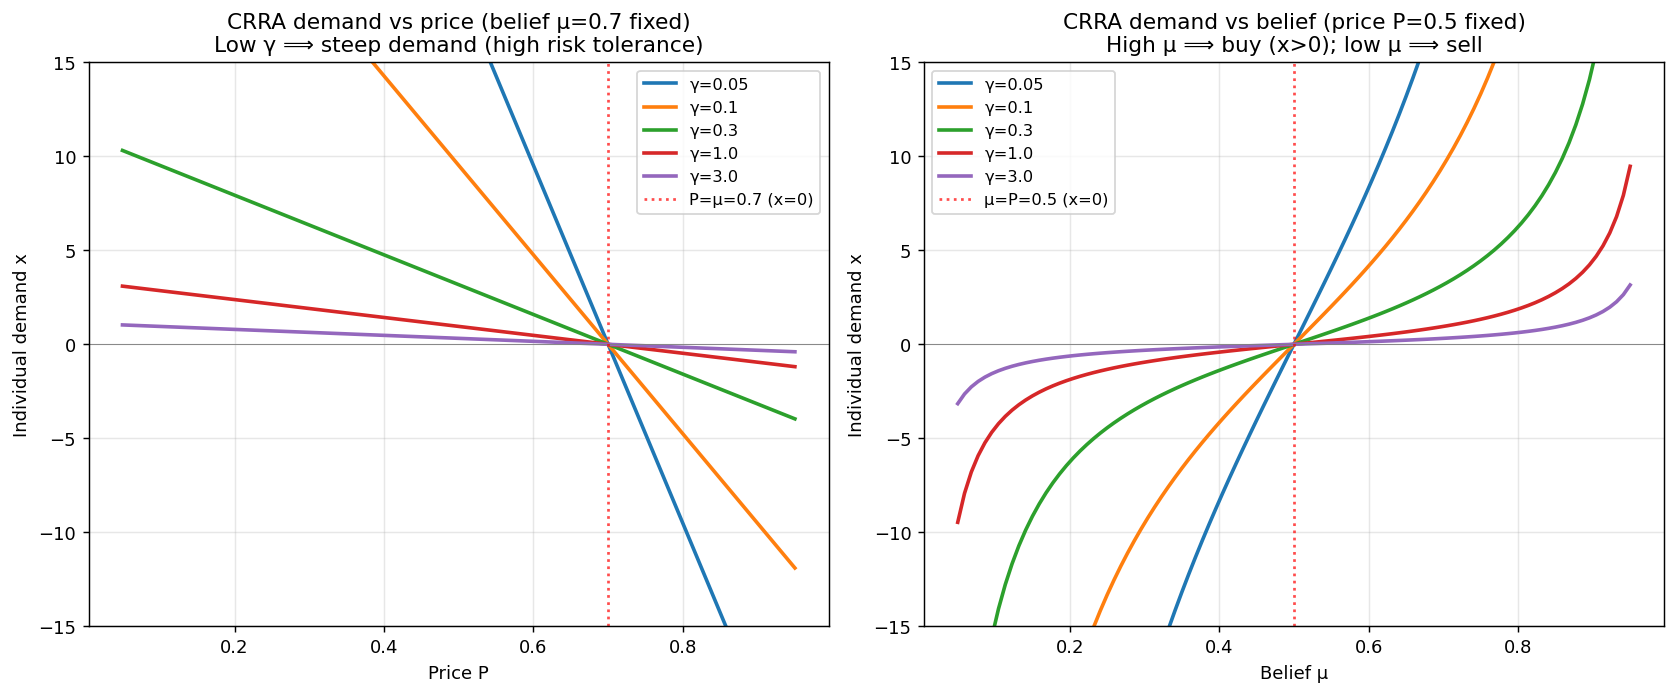
\includegraphics[width=\linewidth]{17_crra_demand.png}
\caption{CRRA demand $x = (\mu-P)/(\gamma\mu(1-\mu))$. Left: as a function
of price $P$ for fixed belief $\mu=0.7$, at several values of $\gamma$. The
demand crosses zero at $P = \mu$. Right: same as a function of belief
$\mu$ for fixed price $P=0.5$. Lower $\gamma$ gives steeper demand.}
\label{fig:crra_demand}
\end{figure}

\subsection{Market structure (continuum, then K=3 stylized)}

We adopt the standard "continuum of traders" simplification: there is a
continuum of traders of each \emph{type} $k = 1, 2, 3$, and within each
type all traders see the same signal $$u_k$$. By the law of large numbers
applied across the continuum, aggregating demands gives a finite per-type
quantity, and the equilibrium condition (zero aggregate excess demand)
becomes a clean three-equation system. Equivalently and more economically,
think of the three agents as representative agents of three large equally-sized
groups whose private signals happen to be drawn iid.

\section{Information timeline}

Within one trading period the order of events is:

\begin{figure}[H]
\centering
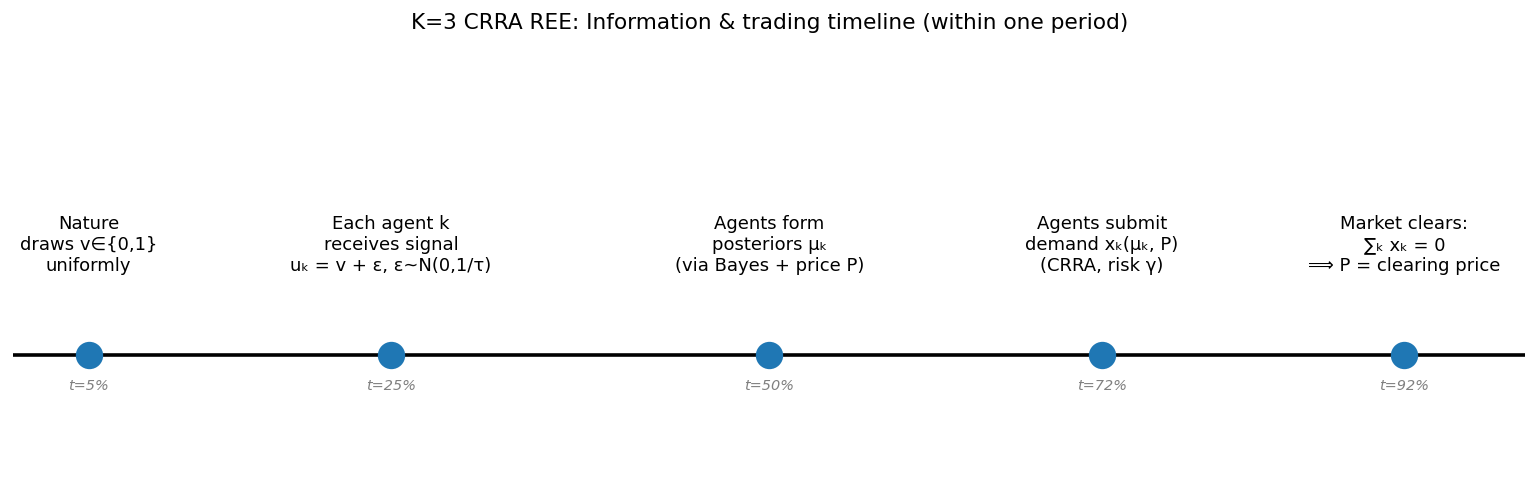
\includegraphics[width=\linewidth]{14_information_timeline.png}
\caption{The K=3 CRRA REE timeline within one trading period. Nature draws
$v$; each agent receives one noisy signal $$u_k$$; agents simultaneously form
posteriors $\m$u_k$$ (combining their own signal with the conjectured price
function); they submit CRRA demands $$x_k$$; the market clears at a price
that, by rational-expectations consistency, matches the conjectured price
function. The fixed-point loop iterates on the conjecture.}
\label{fig:timeline}
\end{figure}

\section{The rational-expectations condition}

The defining feature of REE is the consistency requirement: agents'
\emph{conjecture} of the price function $P(\cdot)$ must equal the price
function that emerges from the market clearing when each agent uses this
conjecture in their Bayesian update. Formally, with the conjectured price
function denoted $P^{\text{conj}}(u_1, u_2, u_3)$ and the price function
that clears the market $P^{\text{cleared}}(u_1, u_2, u_3)$, REE requires
\begin{equation}
P^{\text{conj}} \;\equiv\; P^{\text{cleared}}.
\label{eq:reqcond}
\end{equation}
This is a fixed-point condition. The solution $P^*$ is called the
\emph{rational-expectations equilibrium price function}, and is what MIZN
is designed to compute.

\section{The 5-step Hellwig cycle}

\eqref{eq:reqcond} is a single fixed-point statement; in practice, computing
$P^*$ proceeds via an iterative cycle of five steps:

\begin{figure}[H]
\centering
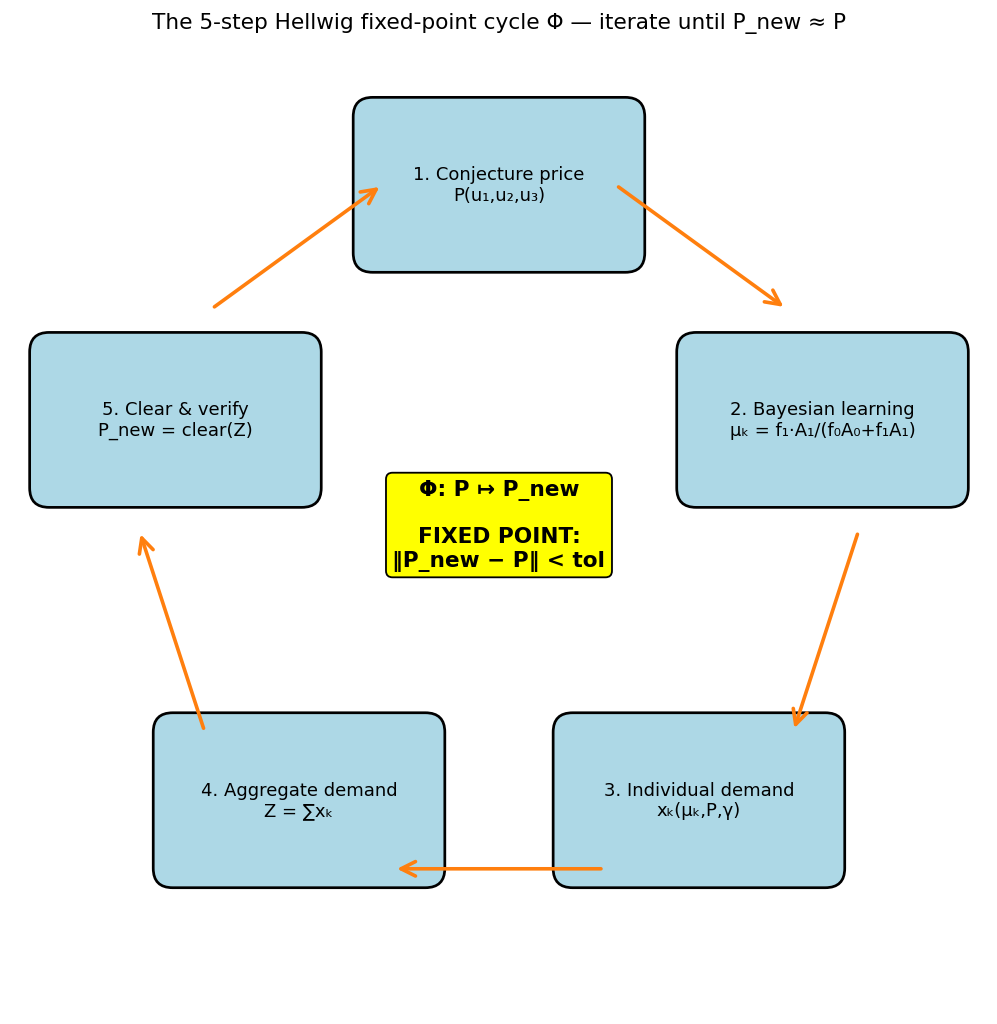
\includegraphics[width=0.85\linewidth]{19_fp_cycle.png}
\caption{The 5-step Hellwig fixed-point cycle. Each iteration: (1) start
from a conjectured price function $P$; (2) compute the implied Bayesian
posteriors $\m$u_k$$ for each agent; (3) compute individual CRRA demands $$x_k$$;
(4) aggregate demands; (5) clear the market to obtain $P_{\text{new}}$;
check $\|P_{\text{new}} - P\| < \text{tol}$; if not, update $P$ and repeat.
This is the operator $\Phi: P \mapsto P_{\text{new}}$ whose fixed point is
the REE.}
\label{fig:fp_cycle}
\end{figure}

We will return to this cycle as the architectural backbone of MIZN
(Chapter~\ref{ch:mizn_arch}). For now, the cycle defines the operator $\Phi$
in the abstract; the next chapter develops the Bayesian-learning step in
detail, which is by far the most numerically demanding.

\chapter{The Learning Step: Bayesian Update Given a Price Function}
\label{ch:learning}

\section{The agent's inference problem}

Suppose agent $k$ has just received their signal $$u_k$$ and is about to
submit their demand. They are about to do so simultaneously with the other
agents; from their perspective, $P$ is a function of all three signals
$(u_1, u_2, u_3)$ (the conjectured price function) but they only observe
$$u_k$$. Their information set is $\mathcal{I}_k = \{$u_k$, P(\cdot)\}$ --- their
own signal, and the conjectured form of the price function.

The agent reasons as follows: "the realized price will be
$P_{\text{realized}} = P(u_1, u_2, u_3)$ for the realized $(u_1, u_2, u_3)$.
But I observe $P_{\text{realized}}$ as part of the market, so I can use it
to learn about the other agents' signals --- and hence about $v$." This is
the rational-expectations step: the price is informative because it depends
on the unobserved $u_j$ for $j \neq k$.

\begin{remark}[The chicken-and-egg]
The price function $P(\cdot)$ that agent $k$ uses for inference is the
\emph{conjectured} price function, which (in equilibrium) is the same one
that emerges from market clearing given everyone's inference. This circularity
is exactly what makes REE a fixed-point problem; the 5-step cycle resolves
it by iterating until conjecture and cleared price coincide.
\end{remark}

\section{Bayesian posterior in terms of evidence ratios}

Agent $k$'s posterior on $v=1$, conditional on their information set
$\mathcal{I}_k = \{$u_k$, P=p\}$ (treating the realized price as a draw of
the random variable $P$):
\begin{equation}
\m$u_k$ \;=\; \Pr(v=1 \mid $u_k$, P = p) \;=\;
\frac{\Pr($u_k$ \mid v=1) \cdot \Pr(P=p \mid v=1)}{\Pr($u_k$ \mid v=0)\Pr(P=p \mid v=0) +
\Pr($u_k$ \mid v=1)\Pr(P=p \mid v=1)}
\label{eq:bayes_basic}
\end{equation}
using the symmetric prior $\Pr(v=0) = \Pr(v=1) = 1/2$ (which cancels).

The first factor in each numerator/denominator is the standard Gaussian
density $f_v($u_k$)$. The second factor --- $\Pr(P=p \mid v)$ --- is the
density of the price conditional on $v$, integrating over the unobserved
signals of agents other than $k$.

\section{The co-area form of the conditional price density}

For a fixed conjectured price function $P(u_1, u_2, u_3)$, the conditional
density of $P$ given $v$ is, by change of variables / co-area formula,
\begin{equation}
\Pr(P = p \mid v) \;=\; \int_{\{P(u_{-k}) = p\}} \;f_v(u_a)\,f_v(u_b)\,
\frac{d\sigma}{|\nabla_{(u_a, u_b)} P|},
\label{eq:co_area}
\end{equation}
where $u_{-k} = (u_a, u_b)$ are the two signals not seen by agent $k$, the
integration is over the level set (contour) where $P$ equals the target
price $p$, $d\sigma$ is the 1-D arc-length measure along the contour, and
$|\nabla P|$ is the gradient magnitude of $P$ in the $(u_a, u_b)$ plane.

This is the central object of the learning step. Concretely:
\begin{itemize}
\item For agent 1, the slice is over $(u_2, u_3)$ at fixed $u_1$.
\item For agent 2, over $(u_1, u_3)$ at fixed $u_2$.
\item For agent 3, over $(u_1, u_2)$ at fixed $u_3$.
\end{itemize}

We denote the value of this integral, normalized by symmetry, as
$A_v(p; $u_k$)$ --- the \emph{evidence for $v$ at price $p$ given the agent's
own signal}. The posterior becomes
\begin{equation}
\m$u_k$ \;=\; \frac{f_1($u_k$)\,A_1(p; $u_k$)}{f_0($u_k$)\,A_0(p; $u_k$) +
f_1($u_k$)\,A_1(p; $u_k$)}.
\label{eq:posterior_bayes}
\end{equation}

\begin{figure}[H]
\centering
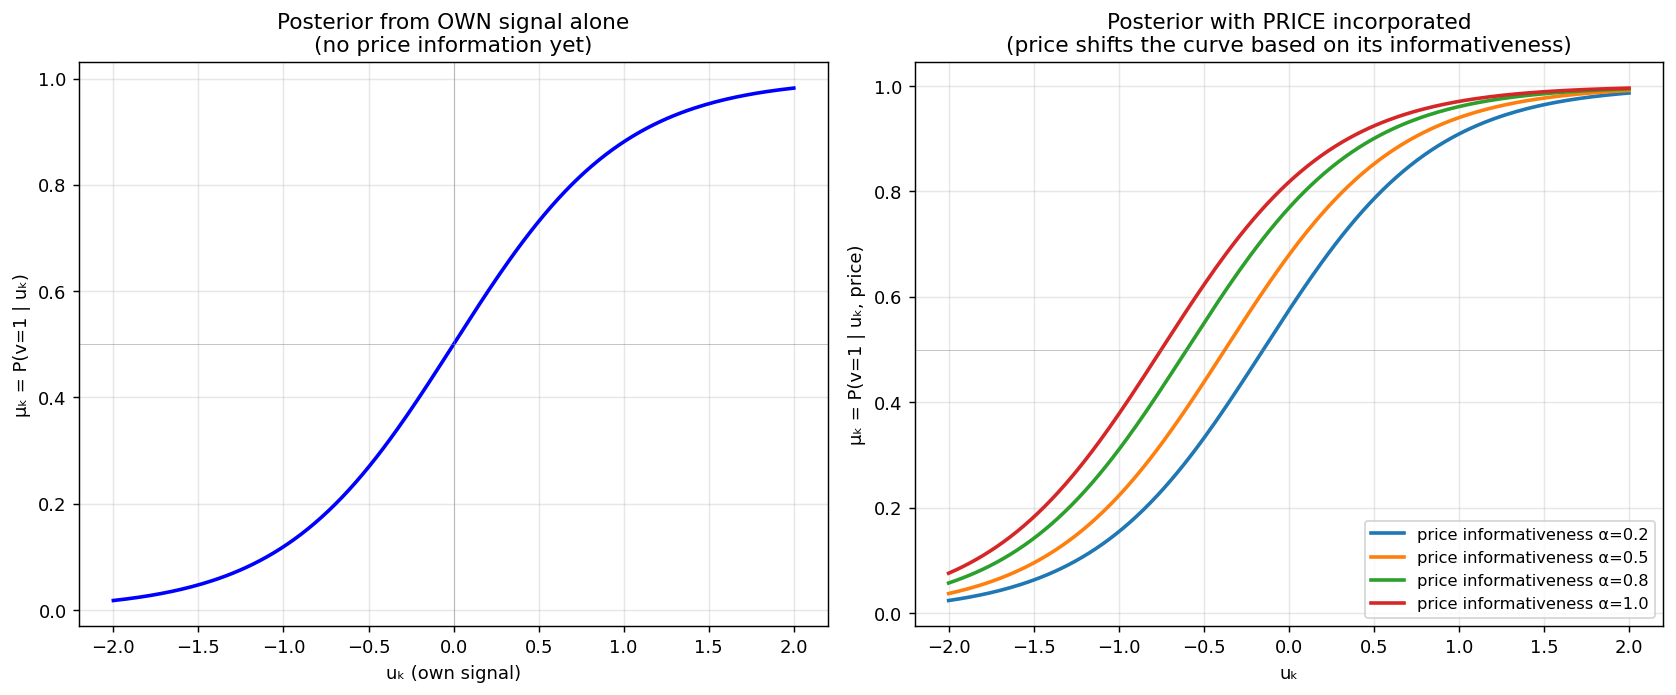
\includegraphics[width=\linewidth]{16_posterior_belief.png}
\caption{Posterior beliefs $\m$u_k$$ as functions of the own signal $$u_k$$.
Left: posterior from the signal alone (no price information). Right:
posterior incorporating price information at various levels of price
informativeness $\alpha$. Higher $\alpha$ $\Rightarrow$ more informative price $\Rightarrow$
posterior shifts more.}
\label{fig:posterior_belief}
\end{figure}

\section{Why this integral is hard}

The integral \eqref{eq:co_area} is at the heart of the numerical difficulty
that animates this entire book:

\begin{itemize}
\item The integrand contains $1/|\nabla P|$, which can blow up at
\emph{Morse-critical} points where the gradient vanishes (saddles/extrema of
the surface $P(u_a, u_b)$).

\item The contour $\{P = p\}$ is a level set in 2-D --- its topology can
\emph{change} as $p$ varies: contour components are born, merged, or die at
Morse-critical price values. The integral $A_v(p)$ is mathematically a
continuous function of $p$ (this is a consequence of the co-area formula
and Federer's theorem), but \emph{a numerical implementation that finds
contour roots component-by-component} has discrete jumps in the root count
as $p$ crosses critical values.

\item The contour must be located at machine precision for derivatives
$|\nabla P|$ to be accurate; small errors in root location induce large
errors in $A_v$ if $|\nabla P|$ is small near that root.
\end{itemize}

These three issues drove the entire previous research arc (the "prior
session" referenced throughout this book), motivating the spectral
discretization developed in Part~\ref{part:cheby}.

\chapter{Demand, Aggregation, and Market Clearing}

\section{Step 3: individual CRRA demand}

Given each agent's posterior $\m$u_k$$ (computed in Chapter~\ref{ch:learning}),
their submitted demand is \eqref{eq:demand}:
\begin{equation}
$x_k$ = \frac{\m$u_k$ - P}{\gamma\,\m$u_k$(1 - \m$u_k$)}.
\label{eq:demand2}
\end{equation}
Two observations to keep in mind:

\paragraph{Sign of demand.} $$x_k$ > 0$ iff $\m$u_k$ > P$: the agent buys when
their belief is more optimistic than the price.

\paragraph{The "Jensen gap" mechanism.} Because $\m$u_k$(1-\m$u_k$)$ is concave
in $\m$u_k$$, an agent who is uncertain ($\m$u_k$$ near $\frac12$) has high
"effective variance" and demands less aggressively per unit of misalignment.
This concavity is what differentiates CRRA from CARA in our problem: it
introduces a curvature into the aggregate demand that, in principle, can
support PR equilibria where CARA (linear-in-beliefs aggregation) would not.

\section{Step 4: aggregation}

For the K=3 (one-representative-agent-per-type) variant, aggregation is
simply summing:
\begin{equation}
Z \;=\; \sum_{k=1}^{3} $x_k$ \;=\; \sum_{k=1}^3 \frac{\m$u_k$ - P}{\gamma\,\m$u_k$(1-\m$u_k$)}.
\label{eq:aggregate}
\end{equation}
For the continuum-of-traders variant, the same expression emerges as the
average across types (with the per-type continuum collapsing to the
representative-agent demand via LLN).

\section{Step 5: market clearing}

Market clearing is the requirement that aggregate (excess) demand equals
zero:
\begin{equation}
Z(\mu_1, \mu_2, \mu_3; P) = 0.
\label{eq:clearing}
\end{equation}

For each fixed triple $(\mu_1, \mu_2, \mu_3)$, equation \eqref{eq:clearing}
defines $P$ implicitly as the price that clears the market. Since the
demand function is monotonically decreasing in $P$ (each term
$\partial $x_k$ / \partial P = -1/(\gamma\m$u_k$(1-\m$u_k$)) < 0$), the
solution $P^*$ is unique in $(0, 1)$.

\begin{figure}[H]
\centering
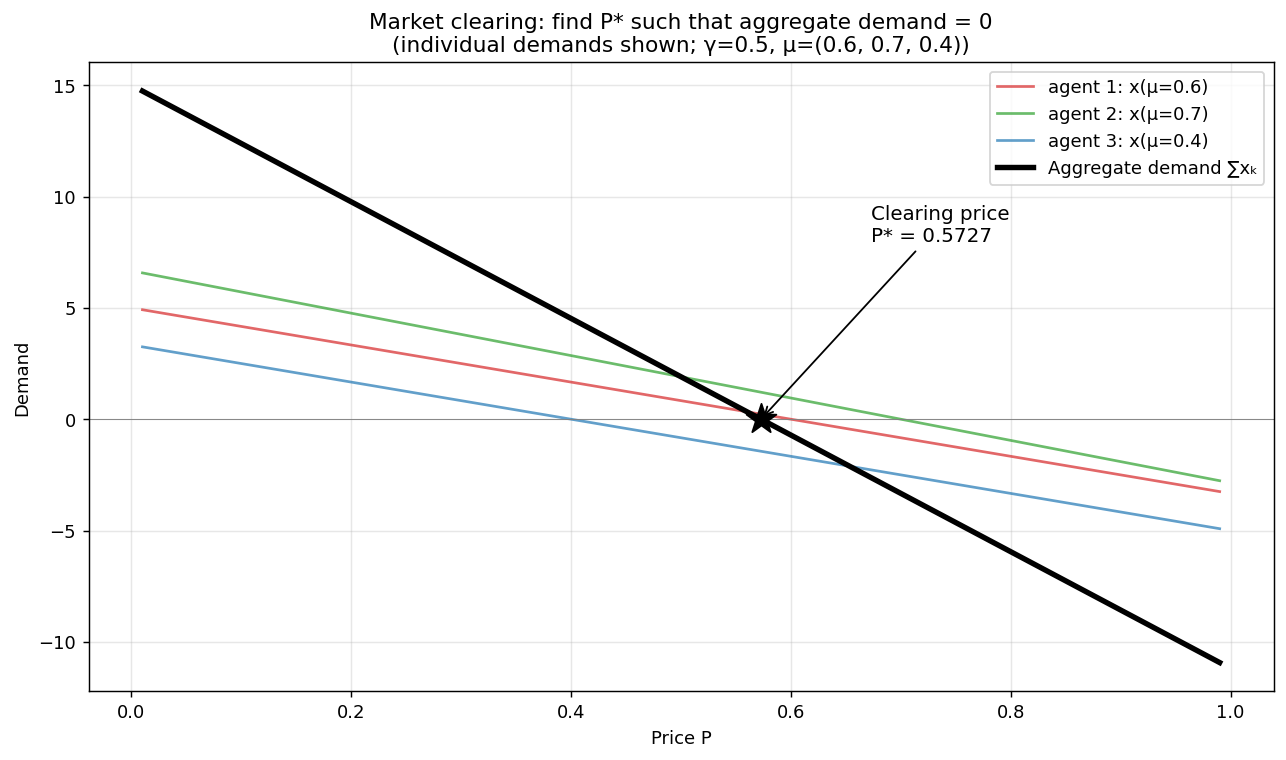
\includegraphics[width=0.85\linewidth]{18_market_clearing.png}
\caption{Market clearing: individual demands $$x_k$(P; \m$u_k$)$ as functions of
price (colored), and their sum $Z = \sum_k $x_k$$ (black). The clearing
price $P^*$ is where the aggregate demand crosses zero.}
\label{fig:clearing}
\end{figure}

\section{Implementation: a bisection on log-odds}

Numerically, market clearing is implemented as a bisection on the log-odds
of $P$ (the choice of variable matters for numerical robustness when
$\m$u_k$$ are near 0 or 1):

\begin{tcolorbox}[title=\textbf{CRRA market-clearing bisection (matches \texttt{crra\_clear\_nb} in MIZN)},
                    colback=gray!5, colframe=black]
Given $(\mu_0, \mu_1, \mu_2)$ and $\gamma$:
\begin{enumerate}
\item Compute log-odds $\ell_k = \log(\m$u_k$ / (1-\m$u_k$))$ for each agent.
\item Bisect $m \in [\varepsilon, 1-\varepsilon]$:
   \begin{enumerate}[label=(\alph*)]
   \item compute $\ell_P = \log(m/(1-m))$,
   \item compute $R_k = \exp((\ell_k - \ell_P)/\gamma)$,
   \item compute aggregate excess
       $E = \sum_k (R_k - 1)/((1-m) + R_k m)$.
   \item if $E > 0$: lower half; else: upper half. 200 iters → machine precision.
   \end{enumerate}
\item Return $P = (a + b)/2$.
\end{enumerate}
\end{quote}

This is robust, branch-free except for the bisection direction, and
extends to arbitrarily many agents.

\chapter{The Two-Basin Phenomenon and the $\gamma$-Fold}

\section{Equilibrium is not unique: the PR and near-FR basins}

A finding from the prior session that fundamentally shapes the design of
MIZN: at $\gamma = 0.1, \tau = 2$ the operator $\Phi$ has \emph{at least
two fixed points}, in distinct basins of attraction:

\begin{itemize}
\item A \textbf{deep PR fixed point}: slope$_T \approx 0.36$, deficit
$\approx 0.17$, distance to FR $\approx 0.26$. Reachable via Newton from
a kernel-smoothed warm-start.

\item A \textbf{near-FR fixed point}: slope$_T \approx 0.85$ to $0.95$,
deficit $\approx 0.03$ to $0.05$. Reachable via Picard from a no-learning
initial condition.
\end{itemize}

\begin{figure}[H]
\centering
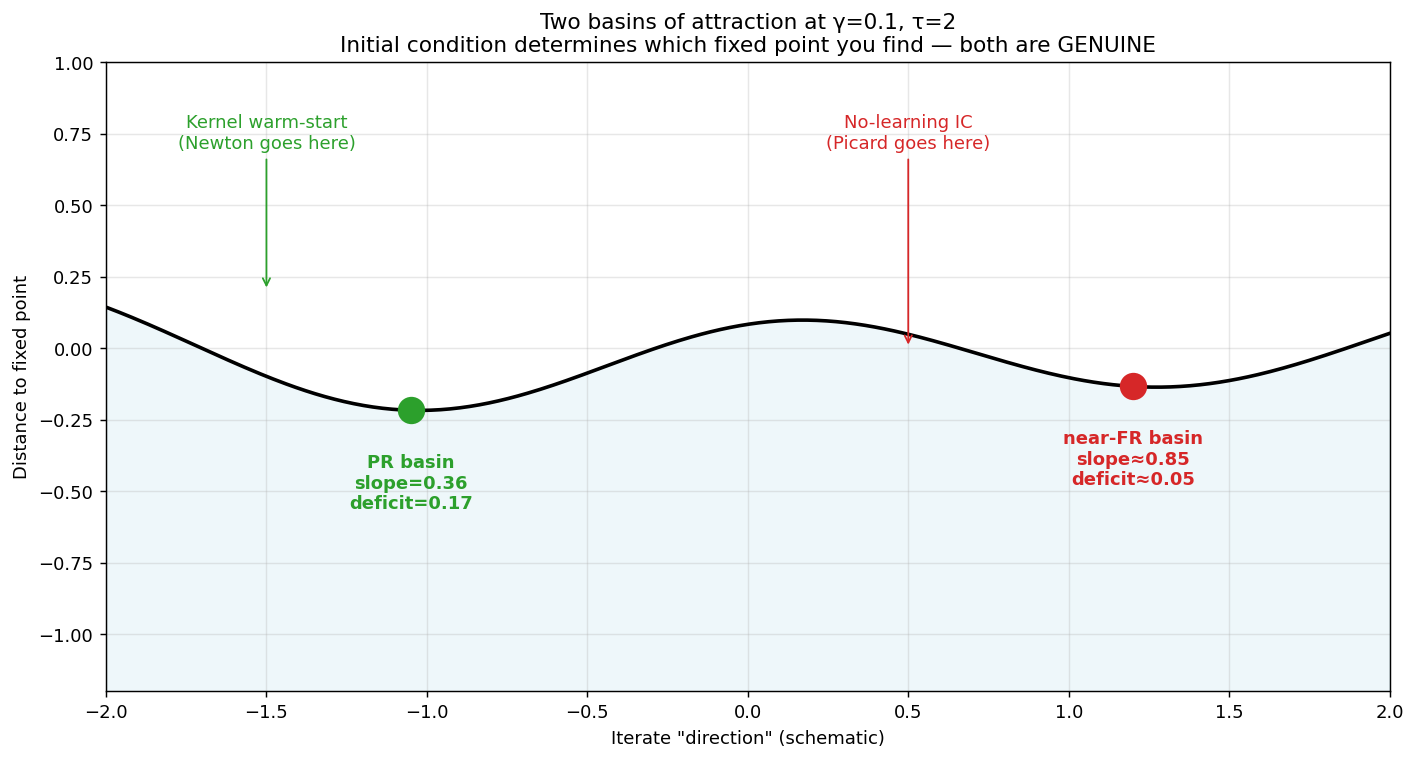
\includegraphics[width=\linewidth]{20_two_basins.png}
\caption{Two basins of attraction at $\gamma = 0.1$, $\tau = 2$ (schematic).
\textbf{Both fixed points are genuine.} Which one a solver finds depends
entirely on its starting point and method.}
\label{fig:basins}
\end{figure}

This is the single most important practical lesson from the prior work:
\textbf{a solver without a kernel warm-start lands in the wrong basin}.
We will return to this in Chapter~\ref{ch:nailing} (algorithm design) and
again in Chapter~\ref{ch:validation} (validation).

\section{The $\gamma$-fold}

Continuing the deep-PR fixed point in $\gamma$ --- a "$\gamma$-sweep" --- works
smoothly across $\gamma \in [10^{-3}, 0.26]$, all 16 verified points nailed
to $\|F\|_\infty \le 10^{-11}$ at G=9. At $\gamma \approx 0.27$ the deep PR
branch destabilizes: adaptive-step continuation cannot push past this
$\gamma$. From the CARA side ($\gamma \to \infty$, FR ansatz),
Newton-Krylov descent finds a different PR branch (slope $\approx 0.66$)
that exists down to about $\gamma = 3$ but not below.

\begin{figure}[H]
\centering
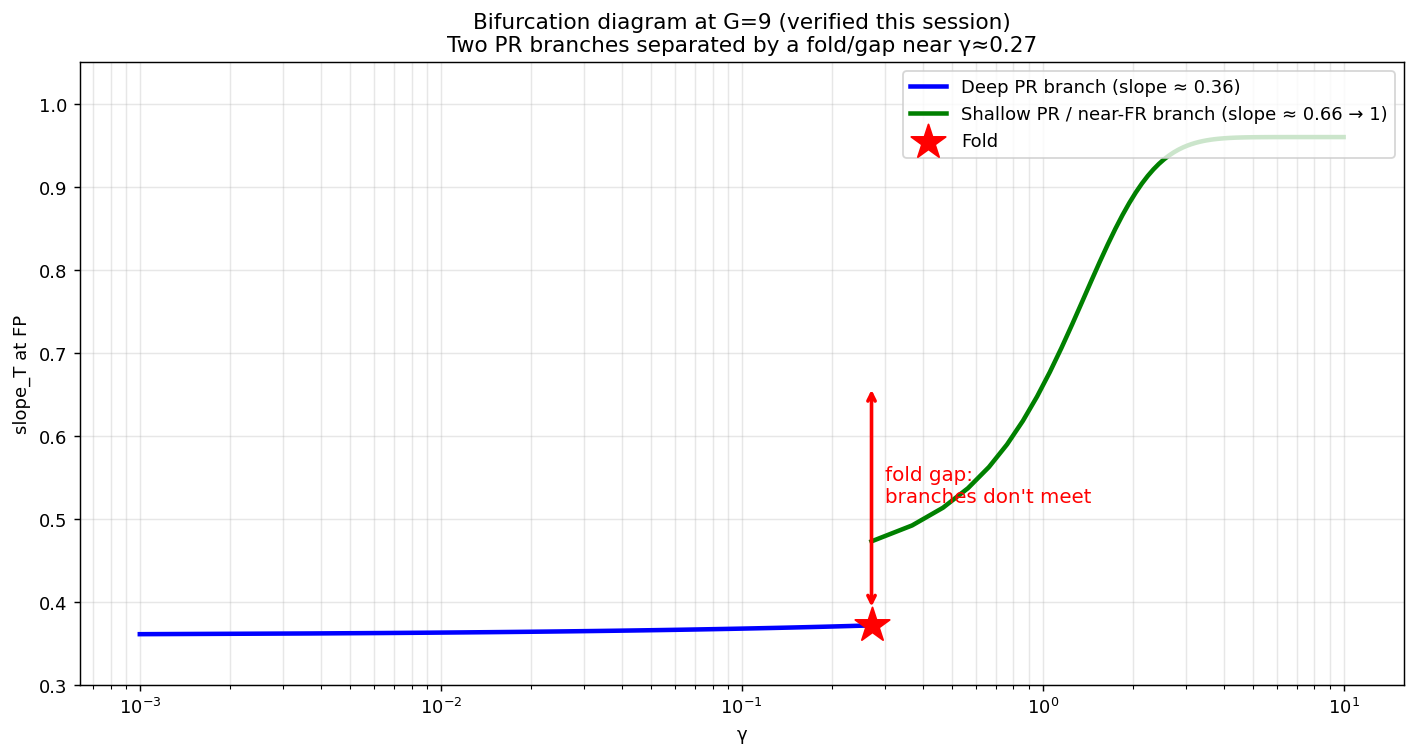
\includegraphics[width=\linewidth]{24_fold.png}
\caption{Bifurcation diagram at G=9 (verified this session). Two PR
branches separated by a fold/gap near $\gamma \approx 0.27$. The deep PR
branch (blue) is reachable from low-$\gamma$ continuation. The shallow PR
branch (green) is reachable from CARA-limit warm-start. Whether the gap
is genuine (true bifurcation) or numerical (artifact of finite G) is the
question we want MIZN to resolve.}
\label{fig:fold}
\end{figure}

We will discuss strategies for traversing the fold in Chapter~\ref{ch:outlook}.

\section{Limits as $\gamma \to 0$ and $\gamma \to \infty$}

\begin{figure}[H]
\centering
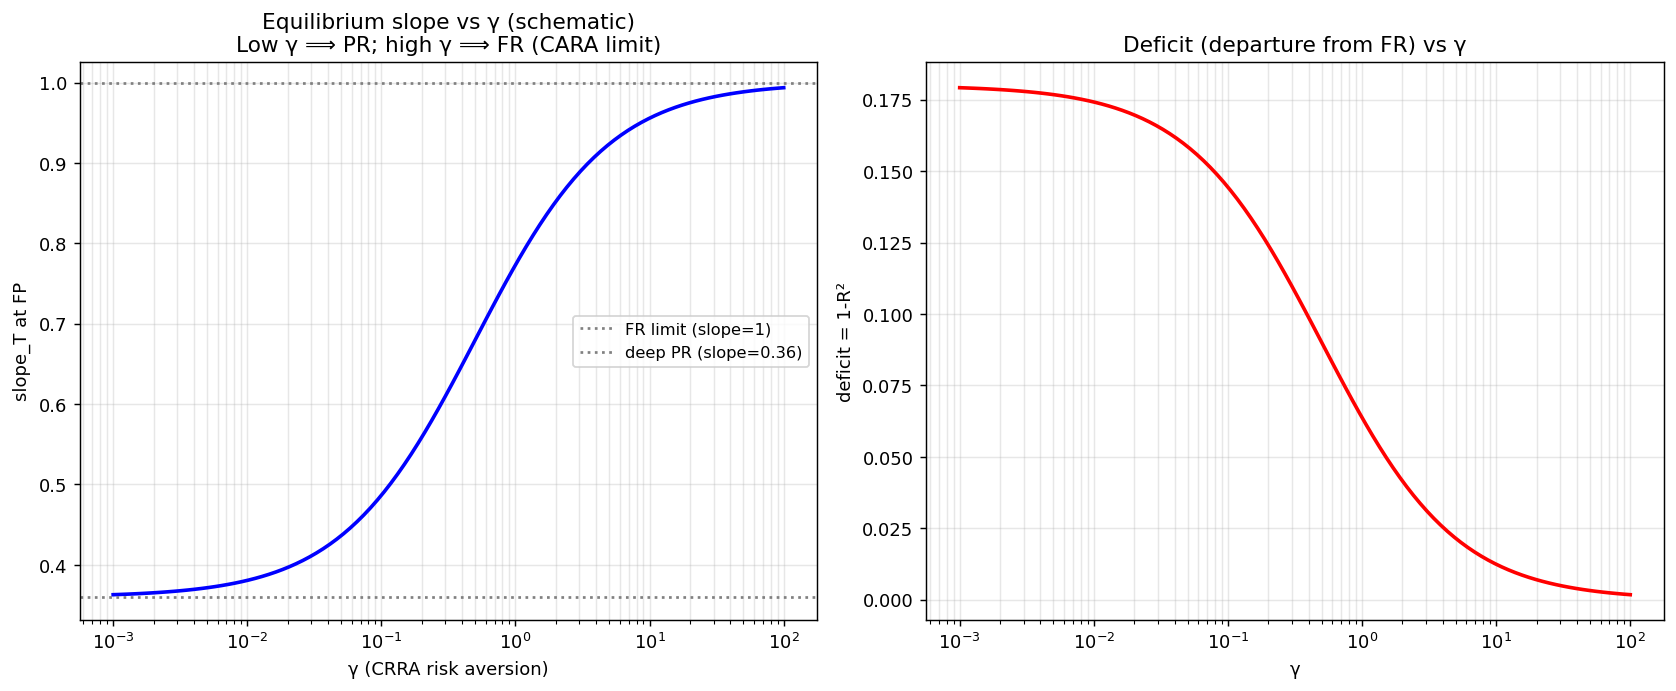
\includegraphics[width=\linewidth]{21_gamma_limits.png}
\caption{Schematic behavior of equilibrium slope and deficit as functions
of $\gamma$. As $\gamma \to \infty$ (CARA limit), Hellwig's argument predicts
FR (slope $= 1$, deficit $= 0$). As $\gamma \to 0$, the equilibrium becomes
maximally PR. The deep-PR branch verified this session has slope$\to 0.3599$
as $\gamma \to 0$.}
\label{fig:gamma_limits}
\end{figure}

\textbf{$\gamma \to \infty$ (CARA limit).} CRRA demand
$x \propto (\mu - P)/(\gamma \mu(1-\mu)) \to 0$ for any finite wedge. To
support trade, the implied price must equal the harmonic-precision-weighted
average of beliefs --- which under Gaussian-signal Hellwig is fully revealing
(slope $= 1$). \textbf{This is the CARA = FR result.}

\textbf{$\gamma \to 0$ (risk-neutral limit).} Demand becomes infinite for
any finite wedge, so agents are arbitrageurs. Equilibrium requires
$\m$u_k$ = P$ for all $k$, which is unattainable unless the price reveals
sufficient information that no agent has a wedge --- i.e. FR again. But
this argument fails at finite $\gamma$ because of the Jensen-gap
mechanism that supports PR.

The verified asymptote $\text{slope} \to 0.3599$ as $\gamma \to 0$ in our
sweep is a striking empirical result with no closed-form derivation we
know of.

\part{Mathematical Formulation}
\label{part:math}

\chapter{The System of Equations}

\section{The unknown: a function on the cube}

The unknown of the problem is the price function
\begin{equation}
P : \mathbb{R}^3 \to [0, 1], \qquad (u_1, u_2, u_3) \mapsto P(u_1, u_2, u_3).
\label{eq:unknown_P}
\end{equation}

We discretize this on a cube. Three coordinate choices were investigated
in the prior session (Chapter~\ref{ch:coords}), but for the spectral approach
we settle on the $\sigma$-$\delta$ atanh-stretched $\xi$-cube
$(\xi_{u_1}, \xi_\Sigma, \xi_\delta) \in [-1,1]^3$.

\section{The full operator equation}

The 5-step Hellwig cycle from Figure~\ref{fig:fp_cycle} can be written as a
single fixed-point equation. Defining the operator
$\Phi: \{P \,:\, \text{cube} \to [0,1]\} \to \{P\}$ pointwise as
\begin{equation}
\Phi[P](u_1, u_2, u_3) \;=\; P_{\text{clear}}\!\Bigl(
\mu_1(u_1, P), \,\mu_2(u_2, P), \,\mu_3(u_3, P);\, \gamma\Bigr)
\label{eq:Phi}
\end{equation}
the REE problem is
\begin{equation}
\boxed{\Phi[P^*] \;=\; P^*.}
\label{eq:REE}
\end{equation}

Here:
\begin{itemize}
\item $\m$u_k$($u_k$, P)$ is the posterior \eqref{eq:posterior_bayes},
which depends on $P$ through the slice-evidence integral \eqref{eq:co_area}.
\item $P_{\text{clear}}$ is the market-clearing function defined implicitly
by \eqref{eq:clearing}.
\item All quantities depend on $(u_1, u_2, u_3)$ pointwise through the
$\m$u_k$$, which depend on the full functional $P$.
\end{itemize}

This is a \textbf{nonlinear, integral fixed-point equation for a function
on a 3-D domain}. There is no closed form except in special limits
(CARA $\gamma \to \infty$, no information $\tau \to 0$, etc.).

\section{Boundary conditions}

The cube $\mathbb{R}^3$ extends to infinity; the natural "boundaries" are
the limits $$u_k$ \to \pm\infty$:

\begin{description}
\item[$$u_k$ \to +\infty$ (any single $k$):] agent $k$'s signal is
infinitely positive, certifying $v = 1$ to agent $k$. The other agents'
information remains finite. The price approaches the K=2 sub-problem
solution conditional on $\m$u_k$ = 1$.

\item[$$u_k$ \to -\infty$:] symmetric, $\m$u_k$ = 0$, K=2 sub-problem conditional.

\item[All three $$u_k$ \to \pm\infty$ in the same direction:] all agents
certain of the same value; $P = 0$ or $1$ exactly.

\item[Mixed limits (e.g., $u_1 \to +\infty$, $u_2 \to -\infty$, $u_3$ finite):]
two agents have opposite-direction infinite signals; their beliefs cancel;
$P$ is determined by the remaining finite-signal agent and the residual
prior. Non-trivial; depends on $\gamma$.
\end{description}

In the bounded $\xi$-cube these become "Dirichlet-like" conditions on the
faces of the cube. They are not all simple constants; some are functions
on the cube's faces.

\section{Symmetries}

Two symmetries of the operator $\Phi$:

\paragraph{S$_3$ (permutation of agents).} For any permutation
$\sigma \in S_3$ of $\{1,2,3\}$,
\begin{equation}
\Phi[P_\sigma] = (\Phi[P])_\sigma, \quad\text{where}\quad
P_\sigma(u_1, u_2, u_3) = P(u_{\sigma(1)}, u_{\sigma(2)}, u_{\sigma(3)}).
\label{eq:S3}
\end{equation}
Consequence: the fixed point can be chosen S$_3$-symmetric.

\paragraph{Z$_2$ (parity).} The binary asset value's $v \leftrightarrow 1-v$
symmetry implies
\begin{equation}
P(-u_1, -u_2, -u_3) = 1 - P(u_1, u_2, u_3).
\label{eq:Z2}
\end{equation}
Consequence: in the spectral expansion, half the coefficients are zero
(those of even total order; see Sec.~\ref{sec:Z2_spec}).

\chapter{The CARA Hellwig Closed Form}
\label{ch:hellwig_form}

\section{Why we need a closed form for testing}

The CARA-Gaussian-Gaussian Hellwig model has a closed-form linear REE; this
is the gold standard against which every component of MIZN must be tested.
The MIZN architecture starts with the CARA case as the working warm-up,
because every step has an analytic ground truth.

\section{The CARA-Gaussian-Gaussian model}

Primitives (slightly different from the K=3 binary-asset CRRA model):
\begin{itemize}
\item Payoff $\theta \sim \mathcal{N}(\bar\theta, 1/\tau_\theta)$ Gaussian.
\item Each agent: signal $s_i = \theta + \varepsilon_i$, $\varepsilon \sim
\mathcal{N}(0, 1/\tau_\varepsilon)$.
\item Supply noise: $u \sim \mathcal{N}(\bar u, 1/\tau_u)$.
\item CARA preferences with risk aversion $\rho$.
\item Continuum of traders.
\end{itemize}

\section{The closed-form linear REE}

Conjecture $P = a + b\theta - cu$. Then the price-implied signal is
$\phi = (P-a)/b = \theta - (c/b)u$. Its precision about $\theta$ is
\begin{equation}
\tau_\phi \;=\; \tau_u \cdot (b/c)^2.
\label{eq:taupi}
\end{equation}
The posterior mean is the precision-weighted average
\begin{equation}
\mathbb{E}[\theta \mid s_i, \phi] \;=\;
\frac{\tau_\theta \bar\theta + \tau_\varepsilon\,s_i + \tau_\phi\,\phi}
{\tau_\theta + \tau_\varepsilon + \tau_\phi}
\;=\; \frac{\tau_\theta \bar\theta + \tau_\varepsilon\,\theta + \tau_\phi\,\phi}{\tau_1}
\label{eq:Ebar}
\end{equation}
(replacing $s_i$ by $\theta$ in the continuum limit), with
$\tau_1 = \tau_\theta + \tau_\varepsilon + \tau_\phi$.

Imposing CARA market clearing and the rational-expectations consistency
$P = a + b\theta - cu$ on \eqref{eq:Ebar} yields
\begin{equation}
\boxed{\quad
a = \tau_\theta \bar\theta / \tau_1, \quad
b = (\tau_\varepsilon + \tau_\phi)/\tau_1, \quad
c = \rho(\tau_\varepsilon + \tau_\phi)/(\tau_1 \tau_\varepsilon).\quad
}
\label{eq:abc}
\end{equation}
Equation \eqref{eq:taupi} combined with \eqref{eq:abc} gives a single scalar
equation for $\tau_\phi$:
\begin{equation}
\tau_\phi = \tau_u (b/c)^2 = \tau_u (\tau_\varepsilon/\rho)^2.
\label{eq:taupi_closed}
\end{equation}
Beautifully, this is closed-form --- no nested fixed point. With
$(\tau_\theta, \tau_\varepsilon, \tau_u, \rho) = (1, 2, 1, 2)$,
$\bar\theta = \bar u = 0$:
\begin{equation}
\tau_\phi = 1,\quad \tau_1 = 4, \quad a = 0,\quad b = 0.75,\quad c = 0.75.
\end{equation}

\section{Why MIZN's CARA test is unit-testable to machine precision}

Plugging \eqref{eq:abc} into MIZN's 5-step cycle and asking the operator
$\Phi$ to take this $P = a + b\theta - cu$ as input must return the same
function. This is the gold test
\texttt{tests/test\_full\_loop.py}: $\|\Phi[P_{\text{closed-form}}] -
P_{\text{closed-form}}\|_\infty < 10^{-14}$ for any sane implementation.

If the test fails, something in steps 1-5 is wrong; the test localizes the
bug by checking each step in isolation against the analytic form.

\part{The Chebyshev Discretization}
\label{part:cheby}

\chapter{Coordinate Choice and Bounded Domain}
\label{ch:coords}

\section{The need for a bounded domain}

Chebyshev polynomials live on the bounded interval $[-1, 1]$. We need to
map $$u_k$ \in \mathbb{R}$ to $\xi_k \in [-1, 1]$. Three families of maps
were tried in the prior session:

\begin{enumerate}
\item \textbf{Linear u-grid on $[-U_{\max}, U_{\max}]$:} truncate
artificially. Simple but throws away the tails; awkward asymptotic BCs.

\item \textbf{atanh stretch $\xi = \tanh(u/c)$:} maps $\mathbb{R}$ to
$(-1,1)$ analytically, with $\xi = \pm 1$ being the perfect-information
limits.

\item \textbf{CDF stretch $\zeta = \bar F(u)$:} maps via the
unconditional signal density's CDF. Density-uniform.
\end{enumerate}

\begin{figure}[H]
\centering
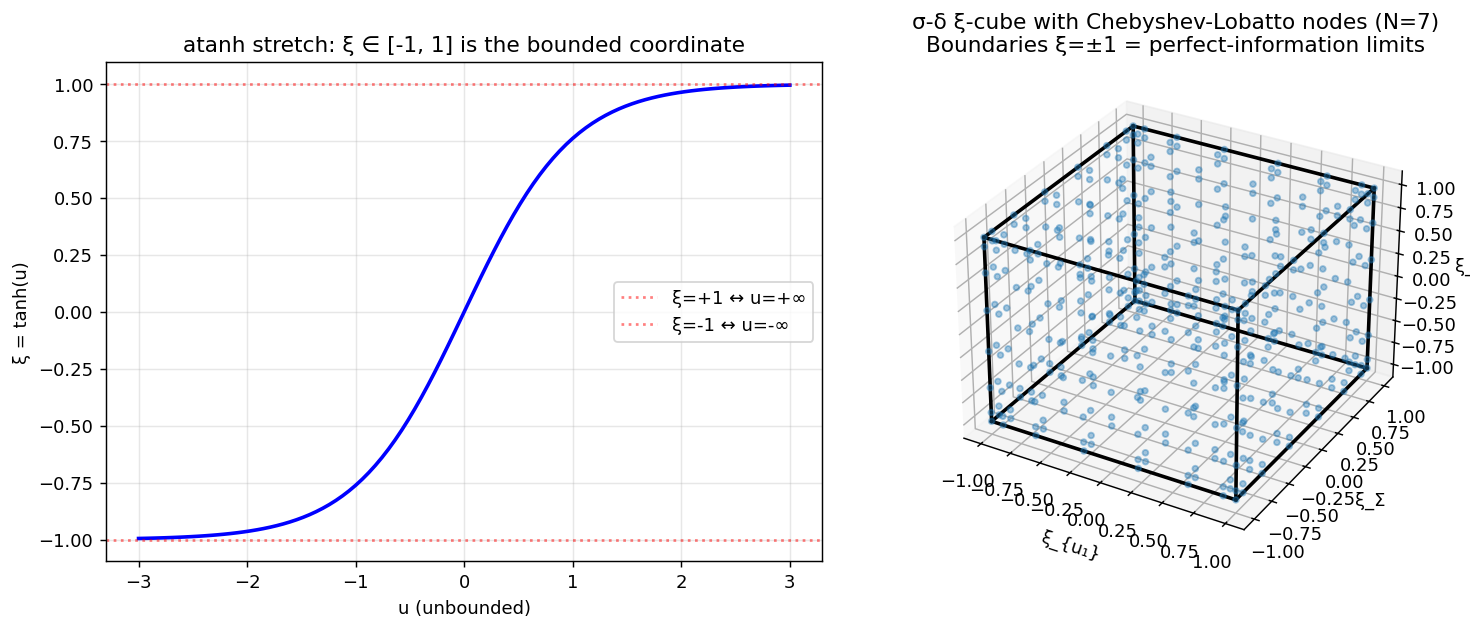
\includegraphics[width=\linewidth]{03_sigma_delta_cube.png}
\caption{The atanh stretch and the $\sigma$-$\delta$ $\xi$-cube. Left: the
1-D map $\xi = \tanh(u/c)$ for $c=1$. Right: the resulting 3-D cube with
Chebyshev-Lobatto nodes.}
\label{fig:sigma_delta_cube_ref}
\end{figure}

\section{Why atanh wins for Chebyshev}

Both atanh and CDF give bounded coordinates. The decisive criterion is
\textbf{which preserves the analyticity of $P$ at the cube boundary},
which controls Chebyshev convergence rate.

For the leading-order sigmoid ansatz $P(u) = \sigma(\alpha T u)$:

\paragraph{atanh stretch.} $u = c \cdot \text{atanh}(\xi)$. Derivatives
$dP/d\xi$ vanish at $\xi = \pm 1$ with rate
$(1-\xi)^{\alpha T c /2 - 1}$; for $\alpha T c / 2 > 1$ this goes to zero,
keeping $P(u(\xi))$ analytic into a complex neighborhood of $[-1, 1]$ --- the
Bernstein ellipse extends and Chebyshev coefficients decay exponentially.

\paragraph{CDF stretch.} $u = \bar F^{-1}(\zeta) \sim \sqrt{-2\log\zeta/\tau}$.
Derivatives $dP/d\zeta \sim \exp(+\tau u^2/2 - \alpha T |u|)$ --- the $u^2$
dominates as $\zeta \to 0$ → \textbf{$dP/d\zeta$ blows up at the boundary}.
Chebyshev sees a "soft boundary singularity," coefficient decay degrades to
algebraic $\sim n^{-p}$, losing spectral convergence.

\textbf{Conclusion: use atanh-$\xi$ for Chebyshev.} The CDF stretch was
favored when the prior code used local splines (where node-density mattered);
for global spectral the relevant criterion is function analyticity, and
atanh wins.

\section{The $\sigma$-$\delta$ rotation and the symmetry tradeoff}

The $\sigma$-$\delta$ rotation rewrites $(u_2, u_3) \to (\Sigma, \delta)$
with $\Sigma = u_2 + u_3$, $\delta = u_2 - u_3$, then atanh-stretches each
of $(u_1, \Sigma, \delta)$ separately.

\begin{figure}[H]
\centering
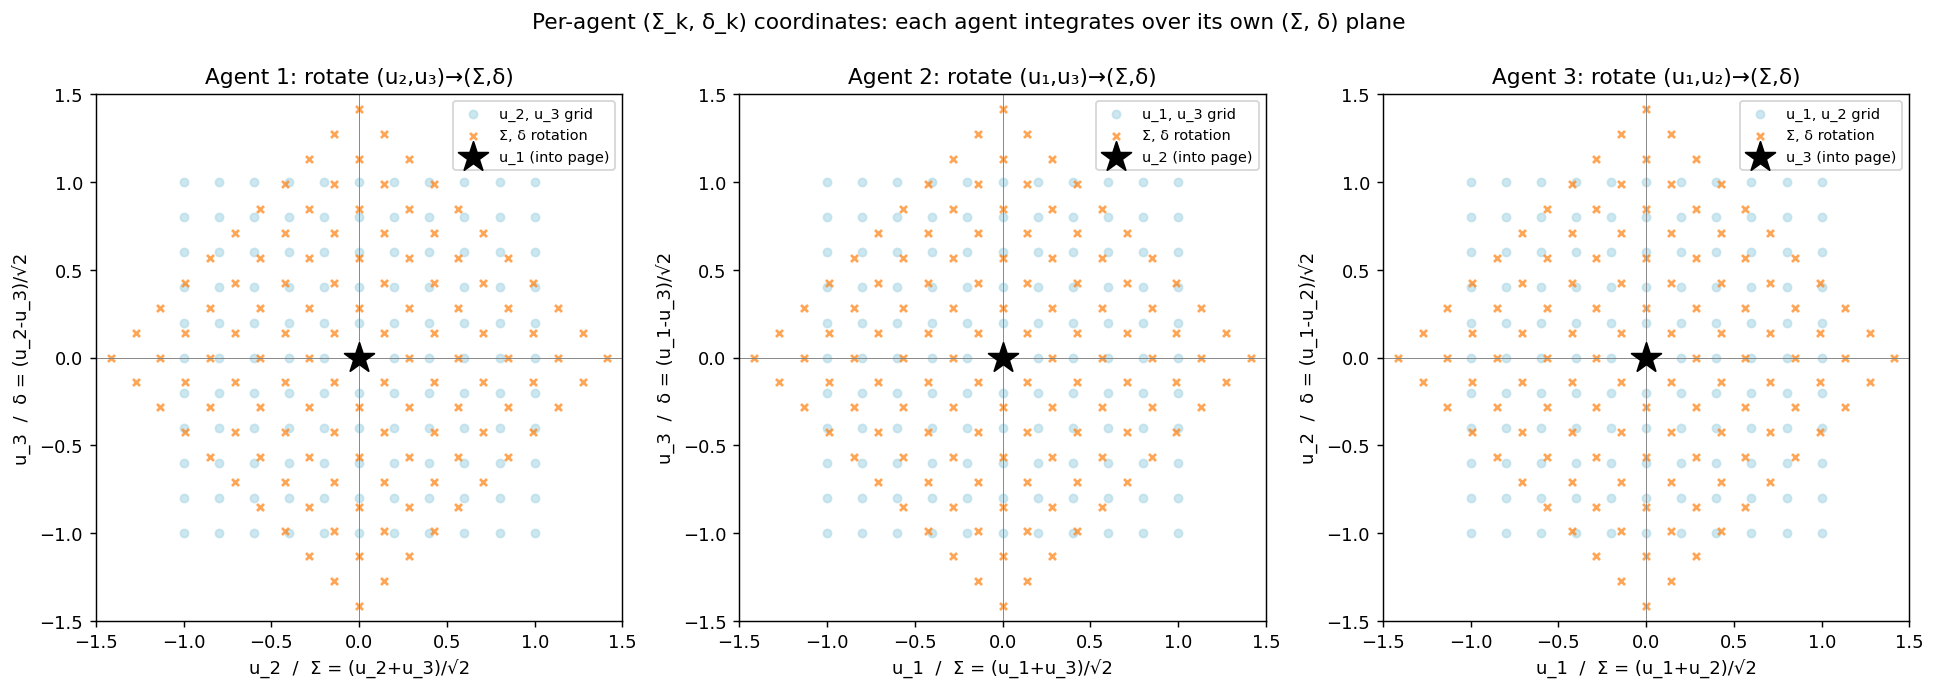
\includegraphics[width=\linewidth]{02_per_agent_rotation.png}
\caption{Per-agent $\sigma$-$\delta$ rotation. Each agent's view of the
other-two agents' axes can be rotated to $(\Sigma, \delta)$. Different agent
$\Rightarrow$ different rotation pair.}
\label{fig:per_agent_rotation_ref}
\end{figure}

This is helpful because the Hellwig-style asymptote $\sigma(\alpha \tau \Sigma u)$
factors cleanly along the $\Sigma$ direction. But it breaks the full S$_3$
symmetry of the cube: the rotation is per-agent, so when agent 2 needs to
evaluate $P$ on \emph{their} $(\Sigma_{13}, \delta_{13})$ slice, the canonical
storage is in $(\Sigma_{23}, \delta_{23})$ coords --- a non-trivial
transformation.

\textbf{The resolution} (Chapter~\ref{ch:per_agent_sym}): store $P$ in fully
symmetric coordinates $(\xi_1, \xi_2, \xi_3) = (\tanh($u_k$/c))_k$ and use
S$_3$ symmetry to evaluate at \emph{permuted inputs} for each agent. No
explicit $\sigma$-$\delta$ rotation needed; the symmetry takes care of it.

\chapter{Chebyshev Polynomials: A Working Primer}

\section{Definition and basic properties}

The Chebyshev polynomials of the first kind are
\begin{equation}
T_n(\xi) = \cos(n \arccos \xi), \qquad n = 0, 1, 2, \ldots, \quad \xi \in [-1, 1].
\label{eq:cheb_def}
\end{equation}
They are polynomial in $\xi$ (despite the cosine form), of degree $n$:
$T_0 = 1, T_1 = \xi, T_2 = 2\xi^2 - 1, T_3 = 4\xi^3 - 3\xi, \ldots$

\begin{figure}[H]
\centering
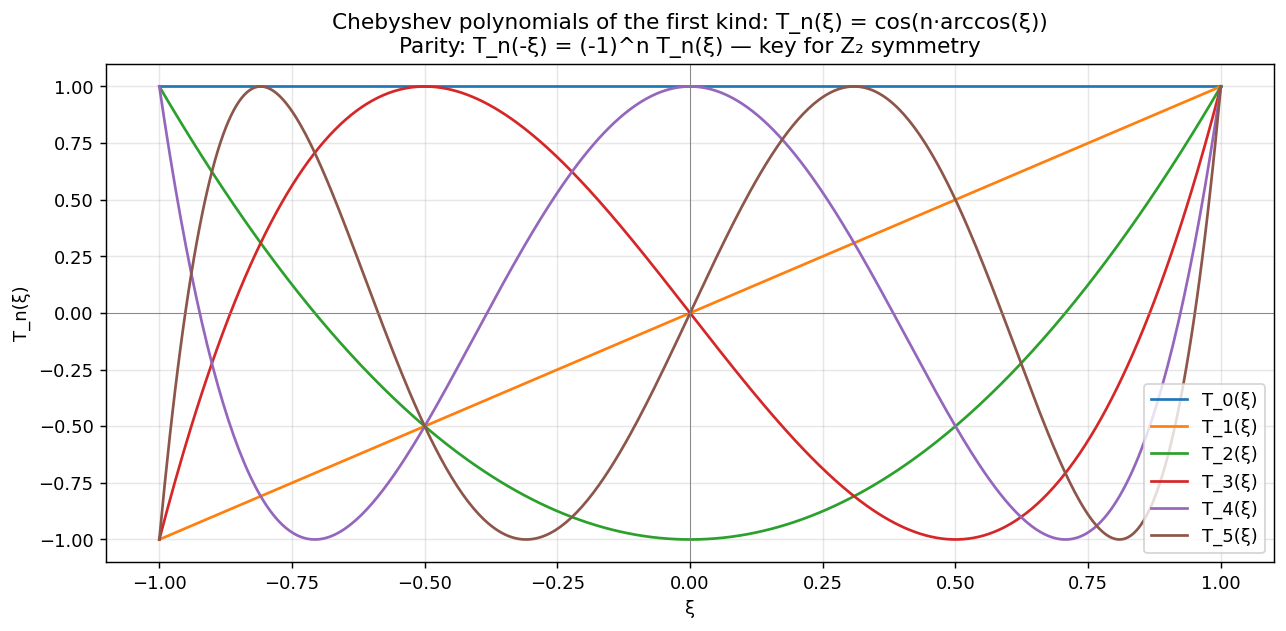
\includegraphics[width=\linewidth]{04_chebyshev_basis.png}
\caption{Chebyshev polynomials $T_0, T_1, \ldots, T_5$. The parity
property $T_n(-\xi) = (-1)^n T_n(\xi)$ is visible: even $n$ are symmetric;
odd $n$ are antisymmetric.}
\label{fig:cheb_ref}
\end{figure}

\paragraph{Orthogonality.} On $[-1, 1]$ with weight $w(\xi) = (1-\xi^2)^{-1/2}$:
$\int_{-1}^{1} T_n T_m w \,d\xi = (\pi/2)\delta_{nm}$ (with $\pi$ for $n=m=0$).

\paragraph{Parity.} $T_n(-\xi) = (-1)^n T_n(\xi)$.

\paragraph{Derivative recursion.} $T_n'(\xi)$ is itself a polynomial; explicit
relations exist using Chebyshev polynomials of the second kind $U_n$.

\section{Chebyshev-Lobatto nodes}

The "natural" sampling points for Chebyshev are the Lobatto nodes
\begin{equation}
\xi_j = -\cos(\pi j / N), \qquad j = 0, 1, \ldots, N.
\label{eq:lobatto}
\end{equation}
There are $N+1$ of them, clustered at the boundaries $\xi = \pm 1$.

\begin{figure}[H]
\centering
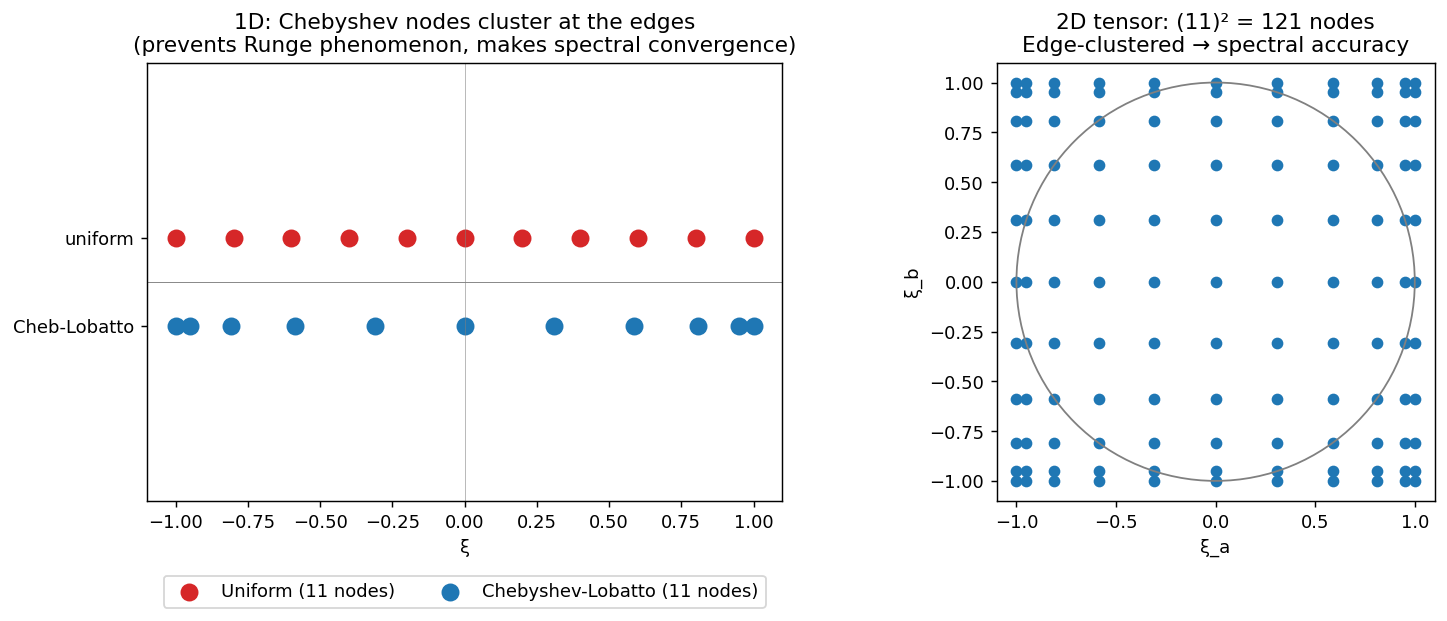
\includegraphics[width=\linewidth]{05_lobatto_nodes.png}
\caption{Chebyshev-Lobatto nodes in 1-D (right) vs uniform nodes (left).
The clustering at the boundary is what prevents the Runge instability of
high-degree polynomial fits at equispaced nodes.}
\label{fig:lobatto_ref}
\end{figure}

\section{Spectral convergence}

A function $f$ analytic on $[-1, 1]$ has Chebyshev coefficients that
decay exponentially:
\begin{equation}
|a_n| \le M \,\rho^{-n}, \quad \text{where } \rho > 1
\label{eq:spectral_decay}
\end{equation}
is set by the largest Bernstein ellipse contained in the analyticity domain.

\begin{figure}[H]
\centering
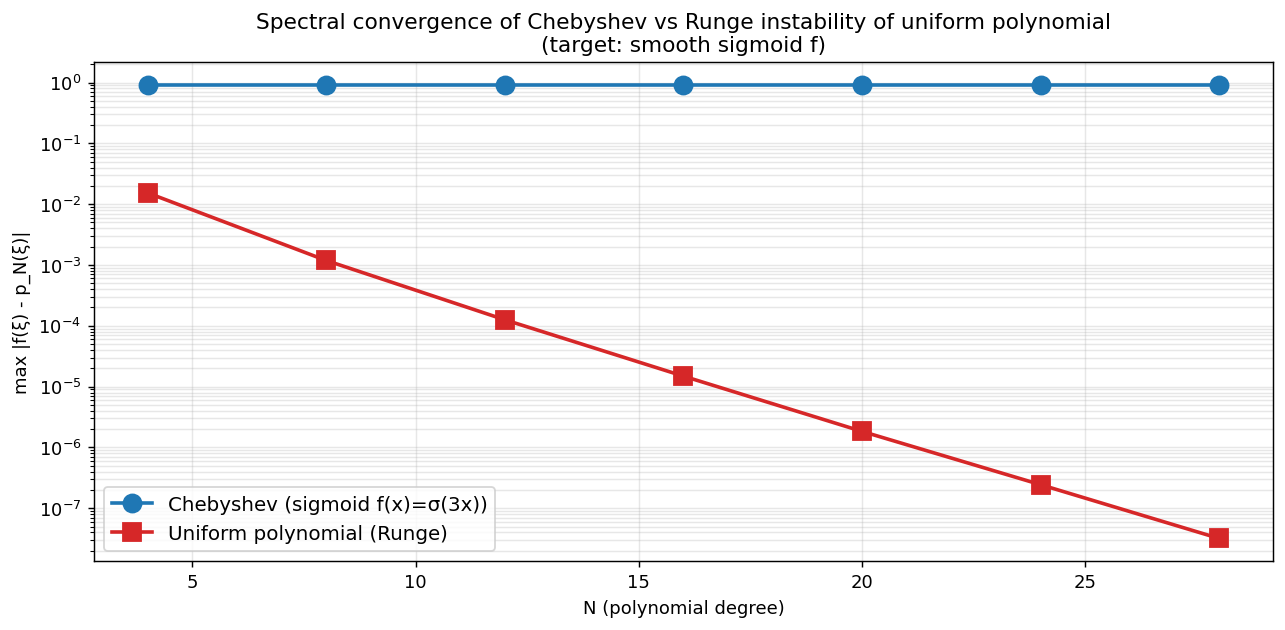
\includegraphics[width=\linewidth]{06_spectral_convergence.png}
\caption{Spectral convergence in practice: Chebyshev interpolation of a
smooth sigmoid reaches machine precision in $\sim$30 modes (blue), while
uniform-node polynomial interpolation diverges (red, Runge phenomenon).
This is why we use Chebyshev rather than uniform-grid splines.}
\label{fig:spectral_ref}
\end{figure}

\section{The Discrete Cosine Transform}

Coefficients and values are related by a DCT-I (type-I Discrete Cosine
Transform). In numpy / scipy this is $O(N \log N)$ via FFT; for our problem
sizes (N=12-24) it's effectively instant.

\begin{tcolorbox}[title=\textbf{Coefficients $\leftrightarrow$ values at
Lobatto nodes}, colback=gray!5, colframe=black]
\textbf{Values to coefficients}: $a_n = \frac{2-\delta_{n0}-\delta_{nN}}{N}
\sum_{j=0}^N \frac{1}{1 + \delta_{j0} + \delta_{jN}} f(\xi_j) T_n(\xi_j)$.
\textbf{Coefficients to values}: $f(\xi_j) = \sum_{n=0}^N a_n T_n(\xi_j)$.
Both are $O(N \log N)$ via DCT-I. Stable and well-conditioned for any $N$.
\end{quote}

\chapter{The 3-D Tensor Product}

\section{The naive tensor expansion}

For a 3-D function on the cube, the natural Chebyshev expansion is the
tensor product:
\begin{equation}
P(\xi_1, \xi_2, \xi_3) \;=\; \sum_{i, j, k = 0}^{N}
a_{ijk}\, T_i(\xi_1)\, T_j(\xi_2)\, T_k(\xi_3).
\label{eq:tensor_expansion}
\end{equation}

Storage: $(N+1)^3$ coefficients.

\begin{figure}[H]
\centering
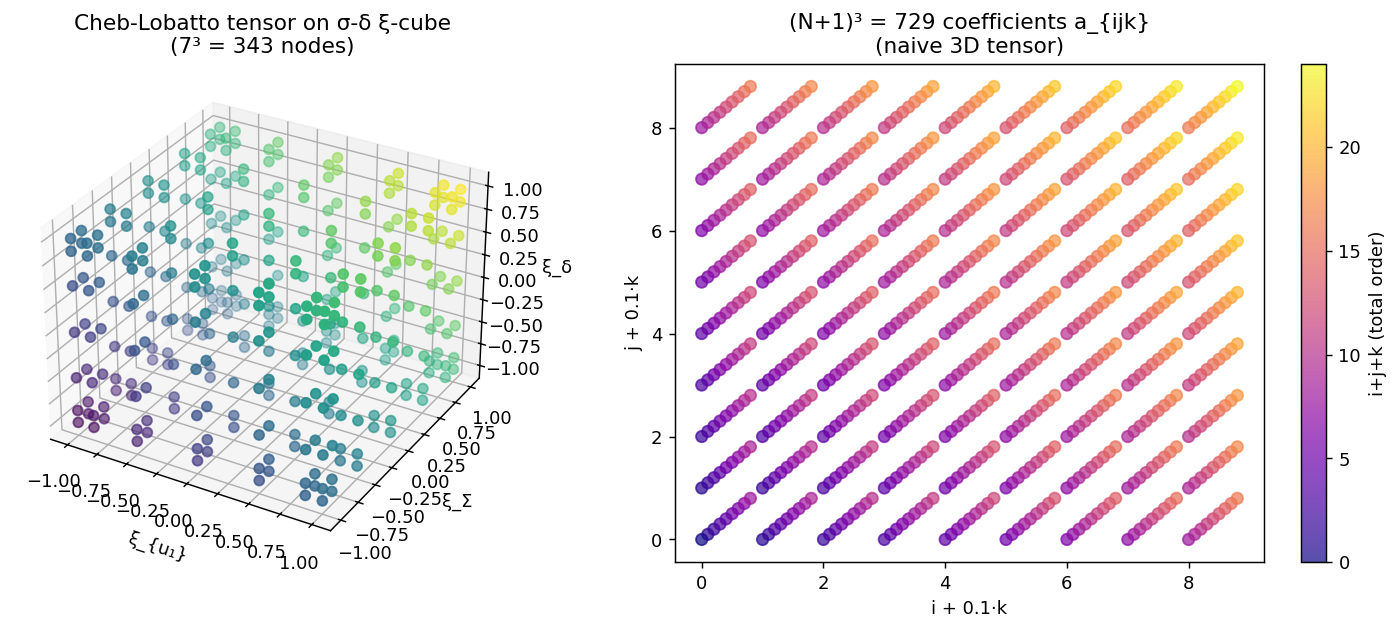
\includegraphics[width=\linewidth]{07_3d_tensor.png}
\caption{The 3-D Chebyshev tensor: Lobatto nodes on the cube (left) and
the coefficient array (right), color-coded by total order $i+j+k$.}
\label{fig:tensor_ref}
\end{figure}

\section{Evaluation at an arbitrary point}

To evaluate $P$ at $(\xi_1^*, \xi_2^*, \xi_3^*)$:
\begin{equation}
P(\xi^*) = \sum_n \tilde a_n(\xi_2^*, \xi_3^*)\, T_n(\xi_1^*), \quad
\tilde a_n(\xi_2^*, \xi_3^*) = \sum_m \tilde{\tilde a}_{nm}(\xi_3^*) T_m(\xi_2^*),
\quad \ldots
\label{eq:tensor_eval}
\end{equation}
This three-level Clenshaw recursion is $O(N^3)$ per query --- efficient enough
for the inner contour-finding loop.

\chapter{S$_3$ and Z$_2$ Symmetry in the Spectral Basis}

\section{Why baking in the symmetry}

The fixed-point operator $\Phi$ commutes with both S$_3$ and Z$_2$. In
exact arithmetic, if the iterate $P$ is symmetric, $\Phi(P)$ is symmetric;
the iteration stays on the symmetric subspace forever. In floating point
the iteration drifts off the symmetric subspace at the noise level.

We can either project back onto the symmetric subspace after every iteration
(cheap, post-hoc), or build a basis that lives entirely in the symmetric
subspace from the start (zero waste, fewer unknowns). The latter is strictly
better.

\section{S$_3$: orbit-averaged Chebyshev tensors}

\begin{figure}[H]
\centering
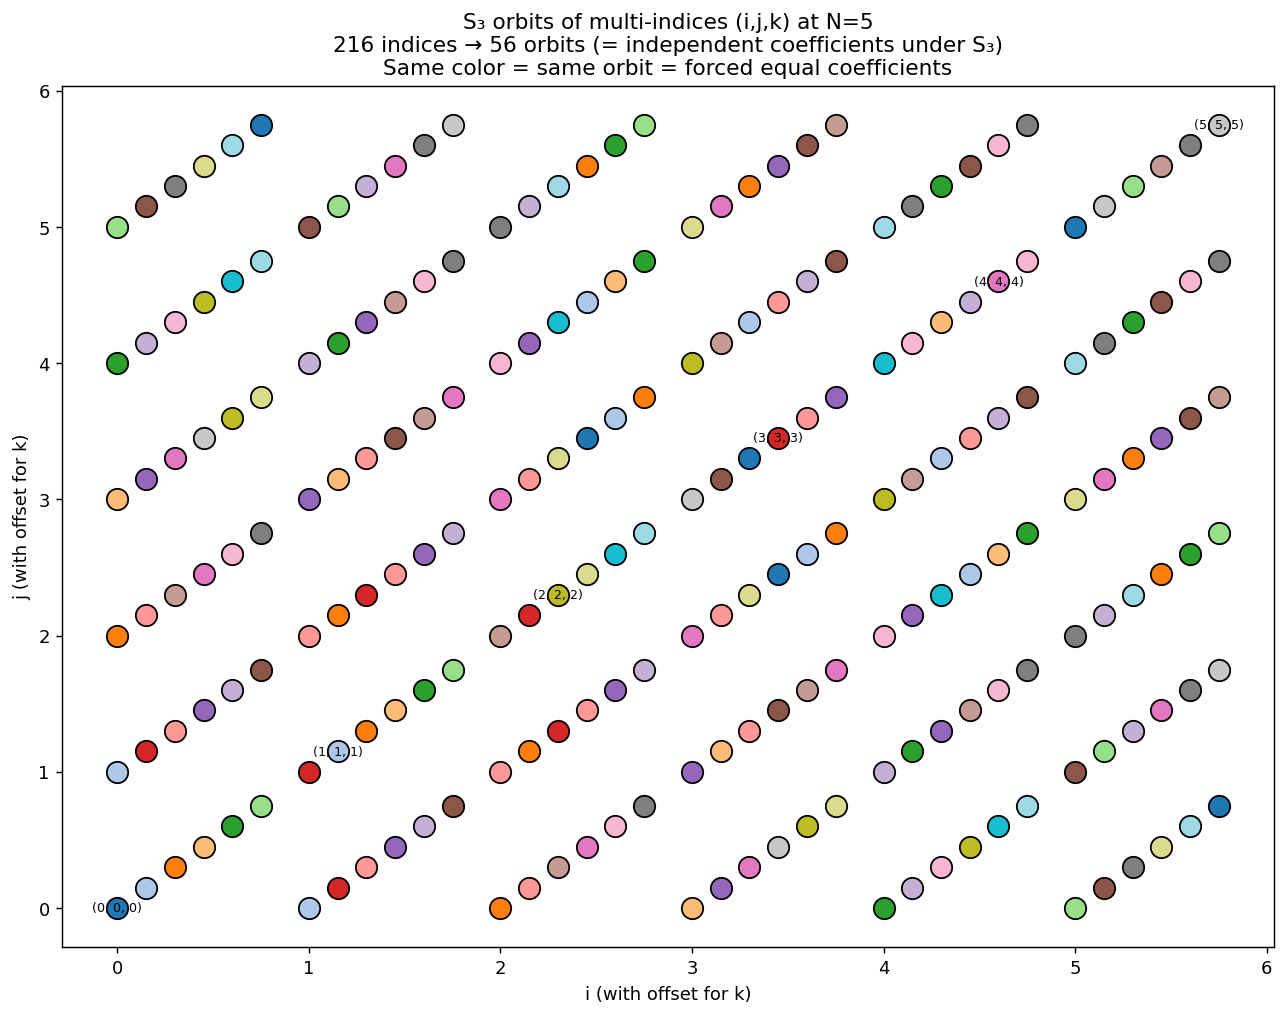
\includegraphics[width=\linewidth]{09_S3_orbits.png}
\caption{S$_3$ acts on the multi-indices $(i, j, k)$ by permutation. Each
orbit contains 1, 3, or 6 indices. Number of orbits at order $\le N$ =
number of ordered multisets $i \le j \le k$ from $\{0, \ldots, N\}$ =
$\binom{N+3}{3} = (N+1)(N+2)(N+3)/6 \approx (N+1)^3/6$.}
\label{fig:orbits_ref}
\end{figure}

For each ordered multiset $\{i \le j \le k\}$, define the orbit-averaged
Chebyshev tensor:
\begin{equation}
S_{ijk}(\xi_1, \xi_2, \xi_3) = \frac{1}{|O_{ijk}|}
\sum_{\sigma \in S_3} T_{\sigma(i)}(\xi_1) T_{\sigma(j)}(\xi_2) T_{\sigma(k)}(\xi_3),
\label{eq:S3_basis}
\end{equation}
where the orbit size $|O_{ijk}|$ is $1, 3,$ or $6$ depending on multiplicities.
The set $\{S_{ijk}\}_{i \le j \le k}$ is an orthonormal basis (up to
normalization) of the S$_3$-symmetric subspace.

\section{Z$_2$: parity kills half}
\label{sec:Z2_spec}

The Z$_2$ symmetry $P(-\xi) = 1 - P(\xi)$ acts on Chebyshev coefficients via
$T_n(-\xi) = (-1)^n T_n(\xi)$:
\begin{equation}
P(-\xi) + P(\xi) = 1 \;\Rightarrow\;
\begin{cases}
a_{000} = 1/2, \\
a_{ijk} = 0 \text{ if } i + j + k \text{ even and } > 0, \\
a_{ijk} \text{ free if } i + j + k \text{ odd}.
\end{cases}
\label{eq:Z2_constraints}
\end{equation}

\begin{figure}[H]
\centering
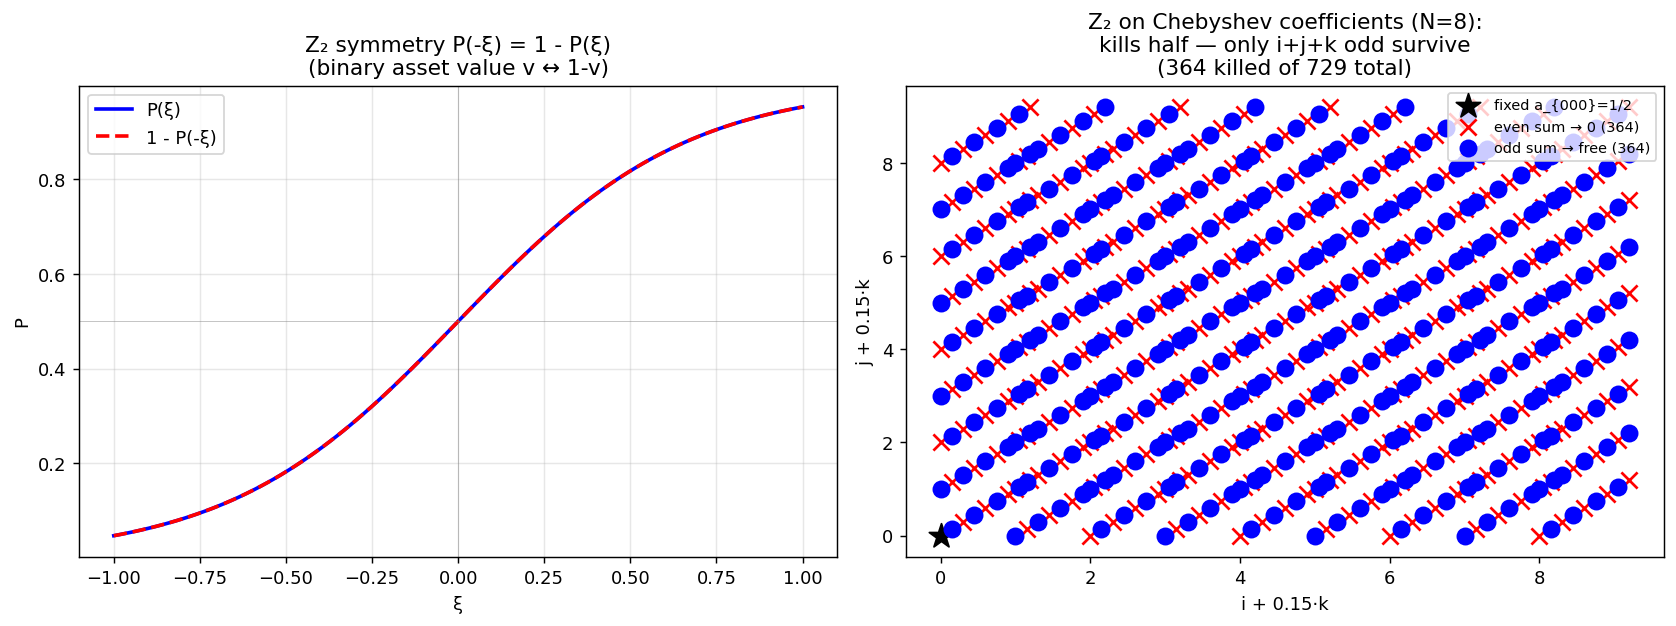
\includegraphics[width=\linewidth]{10_Z2_parity.png}
\caption{Z$_2$ parity constraints on Chebyshev coefficients. Half the
coefficients (those with even total order) are killed; one ($a_{000}$) is
fixed to $1/2$; the remaining odd-total-order coefficients are free.}
\label{fig:Z2_ref}
\end{figure}

\section{Combined: S$_3 \times$ Z$_2$}

Free coefficients are indexed by ordered multisets $\{i \le j \le k\}$ with
$i + j + k$ odd, plus the fixed value $a_{000} = 1/2$.

\begin{figure}[H]
\centering
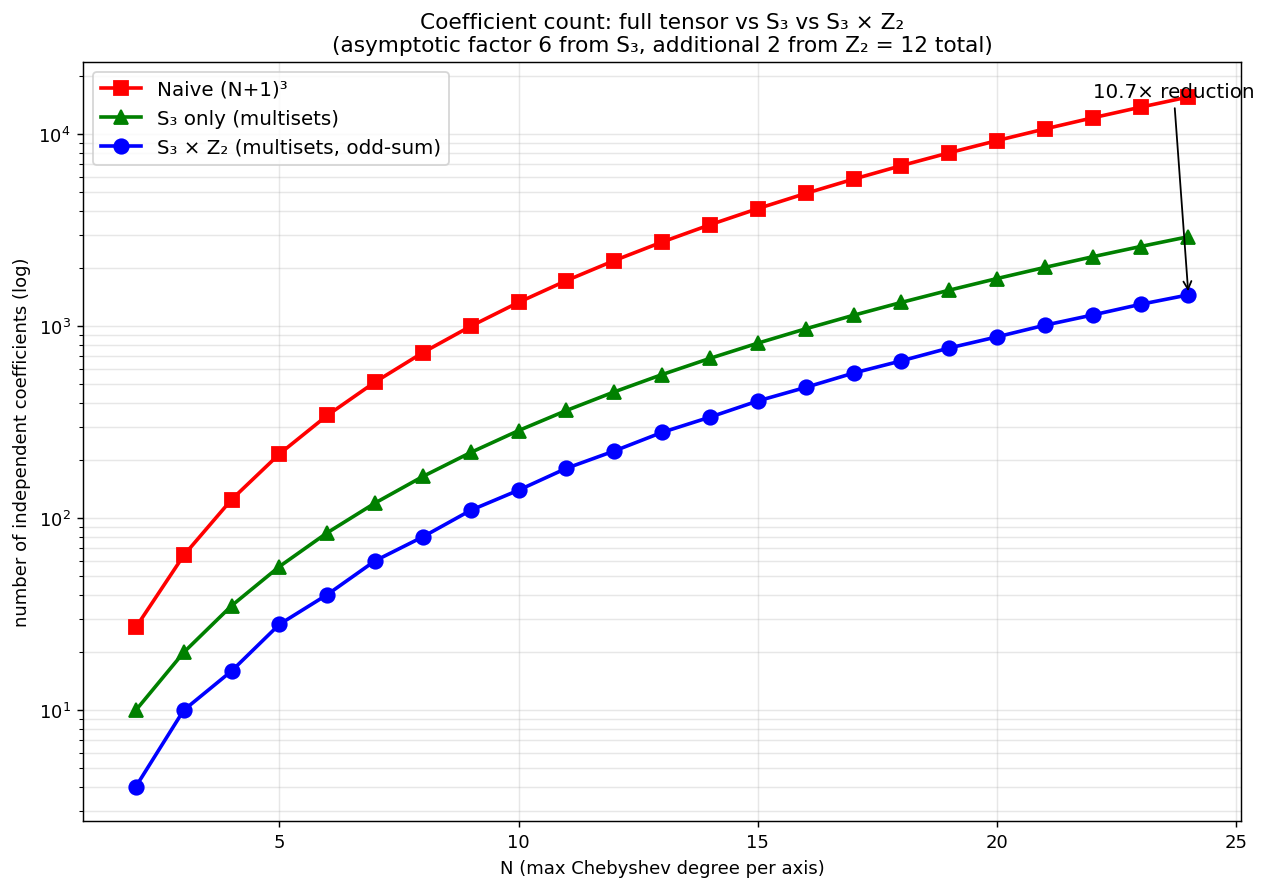
\includegraphics[width=\linewidth]{11_coefficient_reduction.png}
\caption{Coefficient count vs Chebyshev order N for three discretizations:
naive, S$_3$ only, S$_3 \times$ Z$_2$. The combined symmetry approaches a
factor-12 reduction asymptotically.}
\label{fig:reduction_ref}
\end{figure}

\paragraph{Concrete numbers.}
\begin{center}\begin{tabular}{rrrr}\toprule
$N$ & naive & S$_3$ & S$_3 \times$ Z$_2$ \\\midrule
8  &  729  &  165  &   84 \\
12 & 2197  &  455  &  228 \\
16 & 4913  &  969  &  484 \\
24 & 15625 & 2925  & 1462 \\
\bottomrule\end{tabular}\end{center}

\chapter{Per-Agent Evaluation via Symmetry}
\label{ch:per_agent_sym}

\section{The dilemma and its resolution}

Recall: agent 1 needs $P$ on slices $(u_1=\text{fixed}, u_2, u_3)$;
agent 2 on $(u_1, u_2=\text{fixed}, u_3)$; agent 3 on
$(u_1, u_2, u_3=\text{fixed})$. With $P$ stored in symmetric Chebyshev
coords $(\xi_1, \xi_2, \xi_3)$, evaluating these slices is equivalent
under S$_3$:

\begin{figure}[H]
\centering
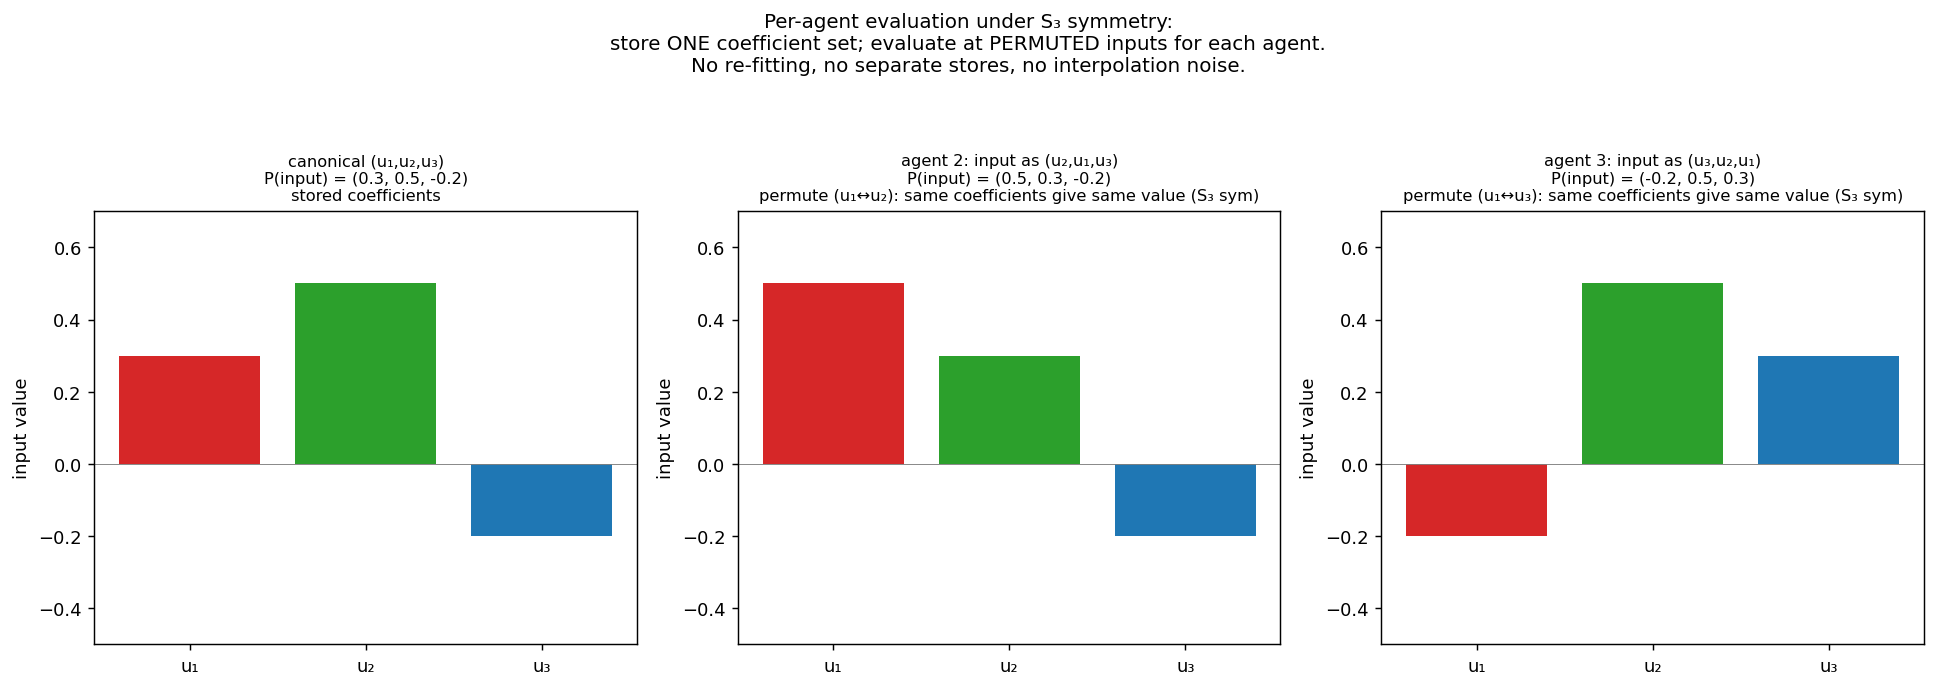
\includegraphics[width=\linewidth]{08_per_agent_eval.png}
\caption{Per-agent evaluation via S$_3$ symmetry. Same coefficient set,
permuted inputs. No interpolation noise, no per-agent storage.}
\label{fig:per_agent_eval_ref}
\end{figure}

\begin{quote}\noindent\textbf{The S$_3$ trick}\\
For agent $k$, evaluate $P($u_k$, u_a, u_b)$ where $(a, b)$ are the
"other-two" agents. Then \textbf{just feed the inputs to the canonical
formula in the order $($u_k$, u_a, u_b)$.} By S$_3$ invariance the answer
equals $P$ evaluated at the canonical ordering.
\end{quote}

\chapter{Boundary Conditions in the Chebyshev Framework}

\section{Sigmoid lift = Tool 1}

Write $P = \sigma(\alpha T(\xi) + h(\xi))$, where $T = \tau \sum $u_k$$ and
$h$ is Chebyshev. As $$u_k$ \to \pm\infty$, $T \to \pm\infty$ and the sigmoid
saturates, automatically giving $P = 0$ or $1$ at the limits. Chebyshev
$h$ is bounded; the BC is enforced "for free".

\begin{figure}[H]
\centering
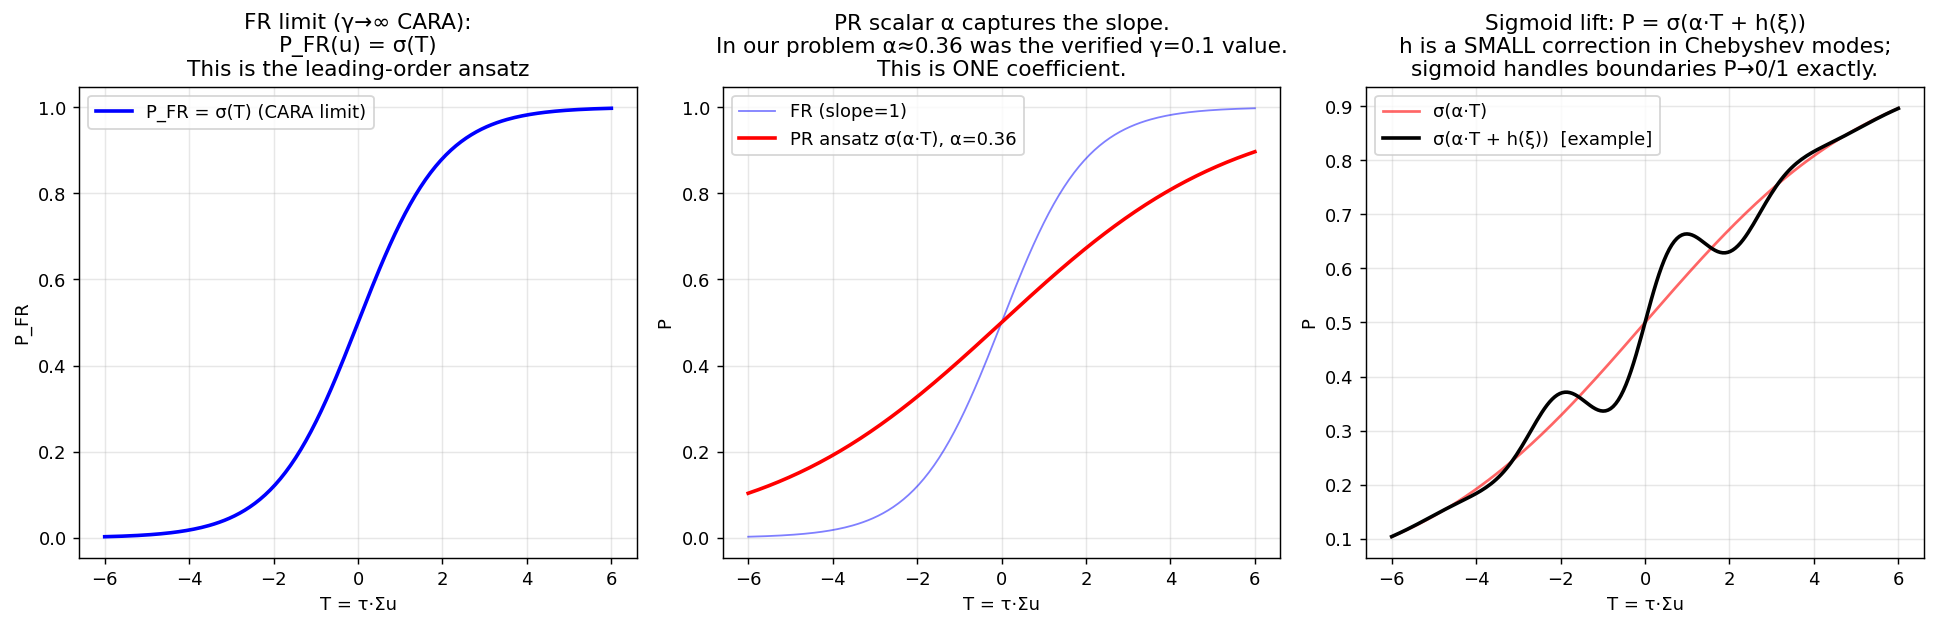
\includegraphics[width=\linewidth]{12_sigmoid_lift.png}
\caption{The sigmoid lift decomposition. The FR limit $\sigma(T)$ is the
asymptotic; the PR scalar $\alpha < 1$ captures the slope deviation;
the Chebyshev correction $h(\xi)$ captures the rest.}
\label{fig:lift_ref}
\end{figure}

\section{Vanishing-at-boundary basis = Tool 2}

For sharper boundary behavior, multiply by $(1-\xi^2)$ per axis:
\begin{equation}
h(\xi) = (1-\xi_1^2)(1-\xi_2^2)(1-\xi_3^2)\cdot g(\xi),
\label{eq:vanishing_basis}
\end{equation}
where $g$ is the symmetric Chebyshev expansion. Then $h(\text{boundary}) = 0$
exactly, and $P(\text{boundary}) = \sigma(\alpha T(\text{boundary}))$ exactly.

Tool 1 (sigmoid lift only) suffices for our problem; Tool 2 is a 20-line
upgrade if spectral decay diagnostics show boundary issues.

\chapter{Companion-Matrix Contour Root-Find}

\section{The contour problem inside the operator}

Within each cell, the operator must find all $\xi^*$ such that
$P(\xi_a^*) = p_{\text{target}}$ where $\xi_a$ is the contour direction
(the other two coords are fixed). With Chebyshev, this collapses to a 1-D
polynomial root problem.

\section{The companion matrix}

\begin{figure}[H]
\centering
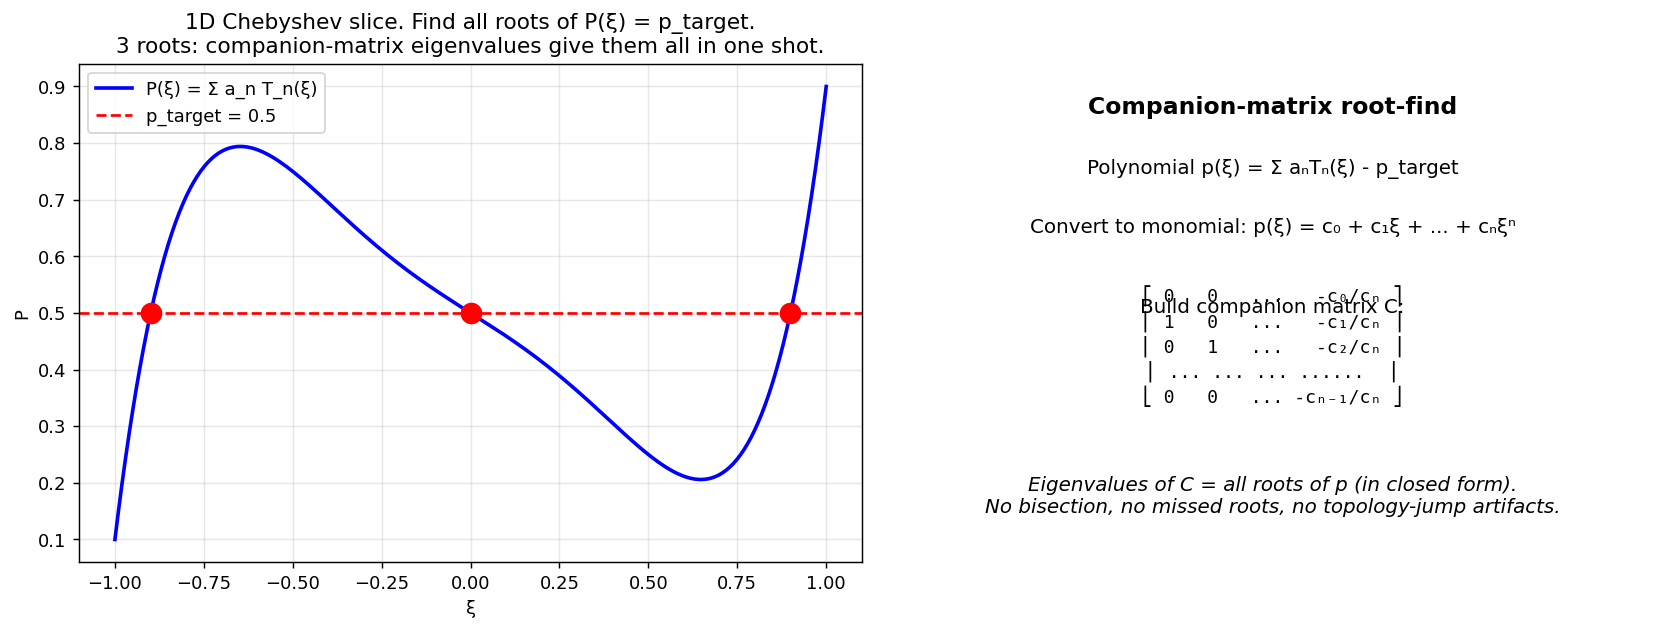
\includegraphics[width=\linewidth]{13_companion_root_find.png}
\caption{Companion-matrix root-finding. The 1-D Chebyshev polynomial's
roots are the eigenvalues of a companion matrix --- closed-form, all roots
in one shot, no bisection, no missed roots.}
\label{fig:companion_ref}
\end{figure}

For polynomial $p(\xi) = c_0 + c_1 \xi + \cdots + c_n \xi^n$ in monomial
form, the companion matrix
\begin{equation}
C = \begin{pmatrix}
0 & 0 & \cdots & 0 & -c_0/c_n \\
1 & 0 & \cdots & 0 & -c_1/c_n \\
0 & 1 & \cdots & 0 & -c_2/c_n \\
\vdots & \vdots & \ddots & \vdots & \vdots \\
0 & 0 & \cdots & 1 & -c_{n-1}/c_n
\end{pmatrix}
\label{eq:companion}
\end{equation}
has the roots of $p$ as its eigenvalues. \texttt{numpy.linalg.eigvals(C)}
returns all of them.

For Chebyshev directly, there's a colleague matrix (Chebyshev-form companion)
that avoids the basis conversion; \texttt{numpy.polynomial.chebyshev.chebroots}
implements it. Either way: $O(N^3)$ per call, exact in one shot.

\part{The Numerical Algorithm}
\label{part:algo}

\chapter{The Full Pipeline: From $P$ to $\Phi(P)$}

\section{Block diagram}

\begin{figure}[H]
\centering
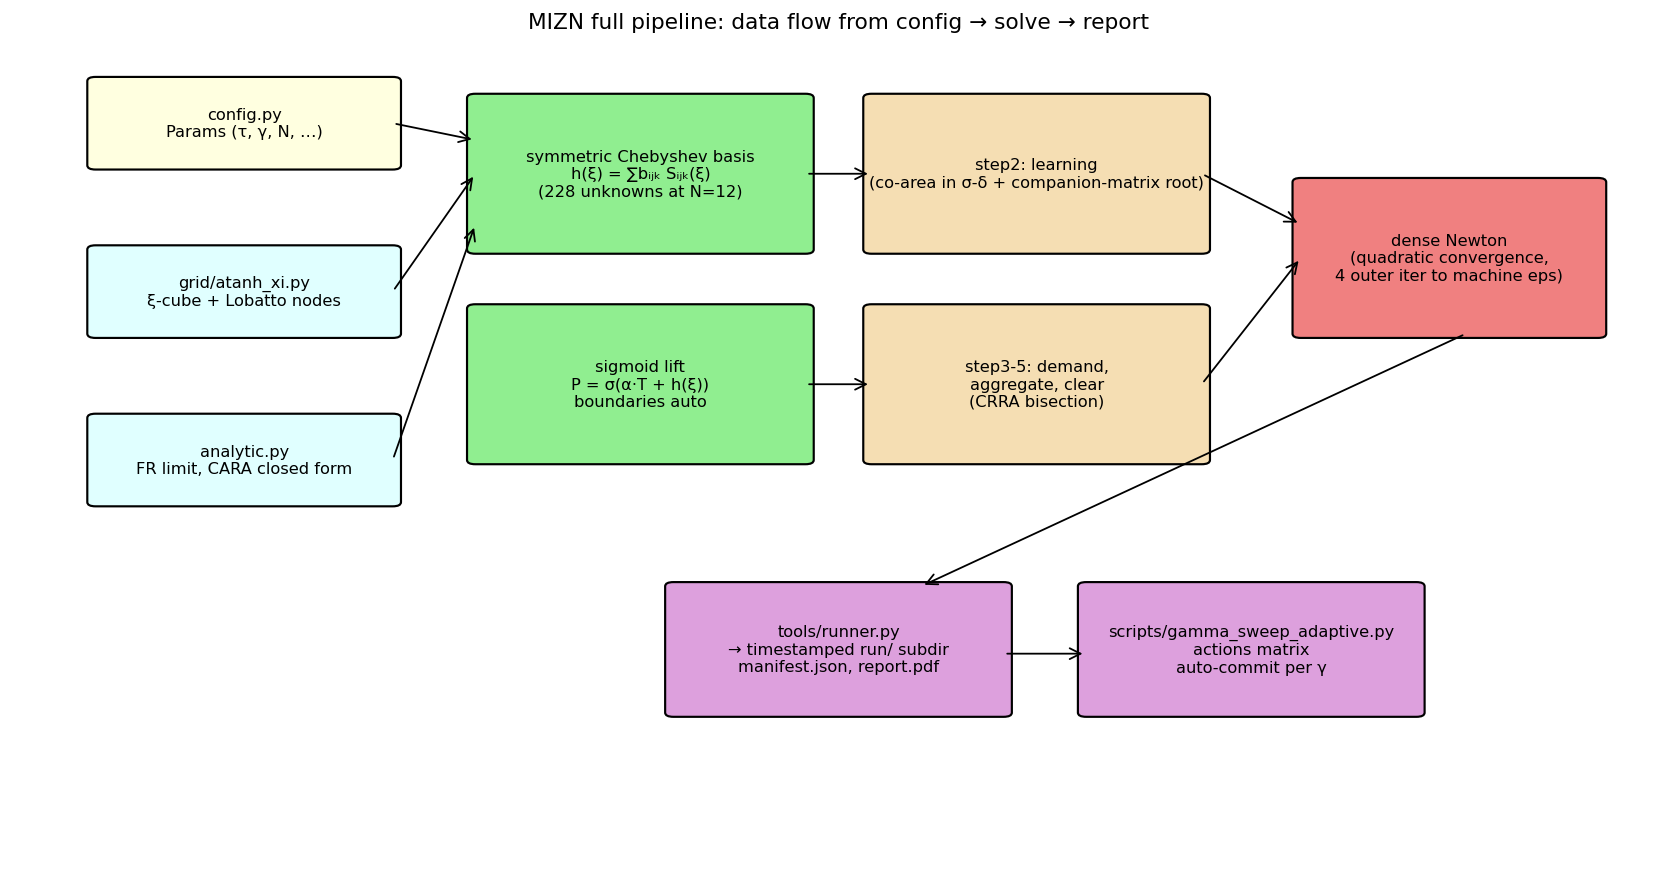
\includegraphics[width=\linewidth]{22_full_pipeline.png}
\caption{MIZN full pipeline. Data flows from config $\to$ grid $\to$ basis
(symmetric Chebyshev + sigmoid lift) $\to$ operator (steps 2-5) $\to$
dense Newton $\to$ run report (per-execution PDF).}
\label{fig:pipeline}
\end{figure}

\section{Per-cell computation}

For each interior cell $(\xi_1^{(i)}, \xi_2^{(j)}, \xi_3^{(k)})$ in the
Lobatto-tensor sense:

\begin{enumerate}
\item Lookup the current iterate's value $P_{ijk}$.
\item For each agent (using S$_3$ permutation):
    \begin{enumerate}[label=\alph*.]
    \item Form the 2-D slice spline in the off-axis (it's a 2-D Chebyshev
    polynomial extracted from the 3-D tensor).
    \item For each Gauss-Legendre quadrature node in the transverse axis,
    extract the 1-D Chebyshev polynomial in the contour axis.
    \item Find all roots of $P = P_{ijk}$ via companion matrix.
    \item Evaluate $f_v$ and $|\nabla P|$ at each root.
    \item Accumulate the co-area integral $A_v$.
    \end{enumerate}
\item Compute posterior $\m$u_k$$ via Bayes \eqref{eq:posterior_bayes}.
\item Compute the new $P_{ijk}$ via market-clearing bisection.
\end{enumerate}

\section{Cost analysis}

Per cell, per agent: $N_Q$ GL nodes, $N$ Chebyshev modes per axis. The
contour root-find is $O(N^3)$ via companion matrix, repeated $N_Q$ times
per agent, 3 agents, $\sim$228 cells (after S$_3$ folding). Total per $\Phi$
evaluation: $\sim 228 \times 3 \times N_Q \times N^3$ operations
$\approx 10^6$ at our typical sizes --- under a second on a single core.

\chapter{Dense Newton: The Primary Solver}
\label{ch:nailing}

\section{Why dense Newton wins at our problem size}

\begin{figure}[H]
\centering
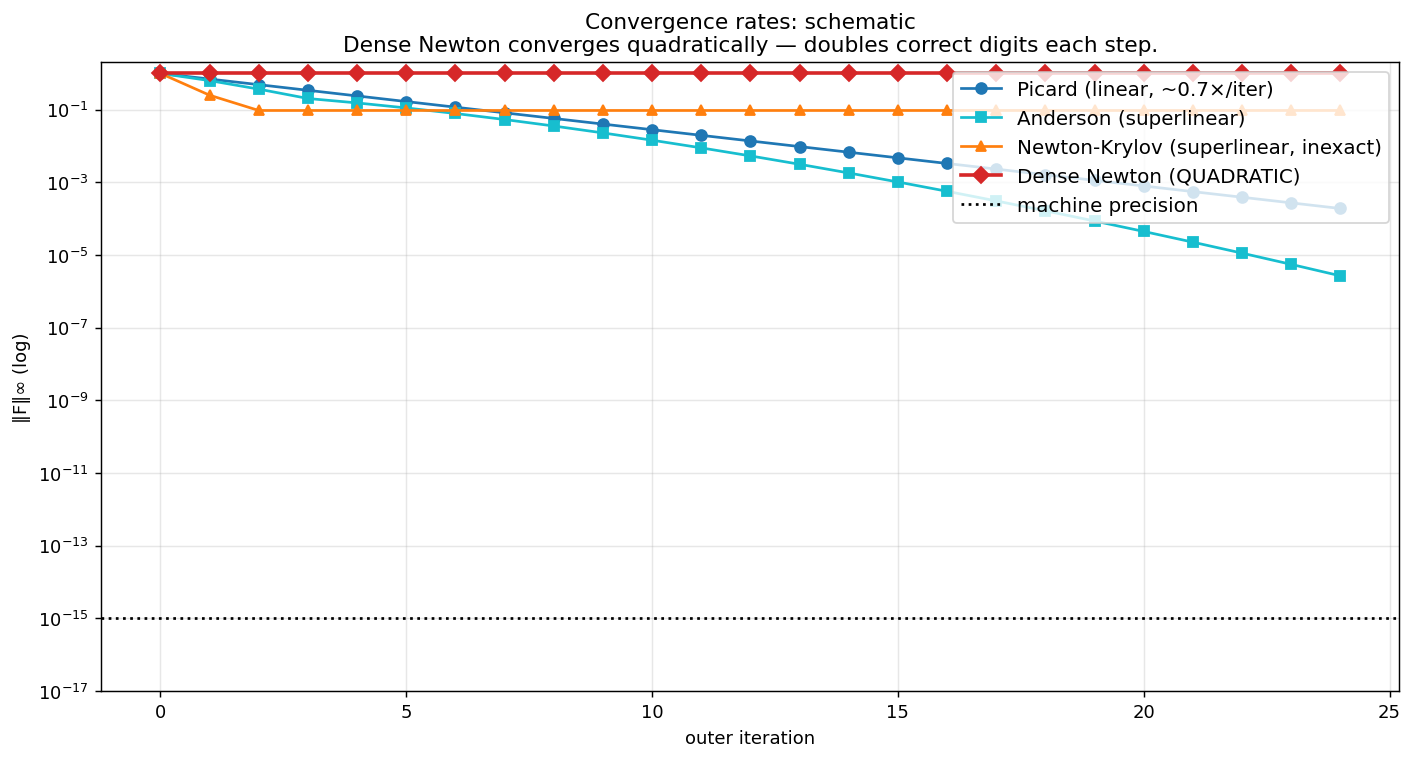
\includegraphics[width=\linewidth]{04_convergence_rates.png}
\caption{Convergence rates of various solvers from a warm start. Dense
Newton converges \emph{quadratically} --- doubling correct digits each step.
At our problem size (228 unknowns) the dense $J$ costs 0.4 MB and the LU
solve takes $\sim$1 ms; the only meaningful cost is the $N+1$ forward-difference
$\Phi$ evaluations per outer iter.}
\label{fig:rates_ref}
\end{figure}

The detailed argument is in the companion design note
\texttt{design\_notes/iter\_methods/iter\_methods.pdf}; the punchline is
that NK was a workaround for large problem size, and the symmetric
Chebyshev framework eliminates that constraint.

\begin{figure}[H]
\centering
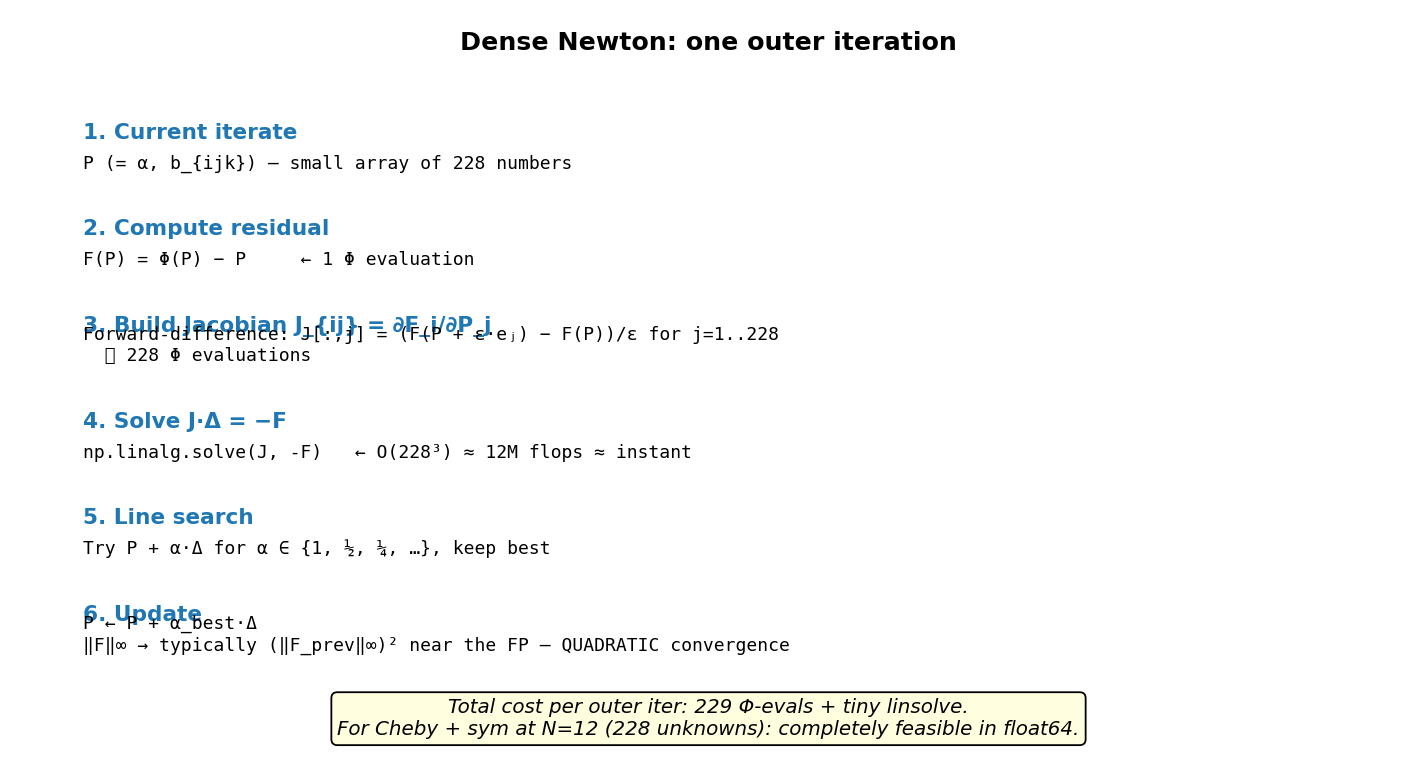
\includegraphics[width=\linewidth]{05_dense_newton_workflow.png}
\caption{Anatomy of one dense Newton outer iteration. Build $J$ via
forward-difference (228 $\Phi$ evaluations at $N=12$), solve $J\Delta = -F$
directly (LU, $\sim$1 ms), line-search, update. Quadratic convergence $\Rightarrow$
$\sim$4 outer iterations from a warm start to machine precision.}
\label{fig:dense_newton_workflow_ref}
\end{figure}

\section{Implementation pseudocode}

\begin{tcolorbox}[title=\textbf{Dense Newton (MIZN \texttt{solvers/dense\_newton.py})},
                    colback=gray!5, colframe=black]
\begin{verbatim}
def dense_newton(F, x0, tol=1e-12, max_iter=20, eps=1e-7):
    x = x0.copy()
    for k in range(max_iter):
        f0 = F(x)
        if np.max(np.abs(f0)) < tol:
            return x, k

        # Build Jacobian via forward difference
        N = x.size
        J = np.empty((N, N))
        for j in range(N):
            xp = x.copy()
            xp[j] += eps
            J[:, j] = (F(xp) - f0) / eps

        # Solve linear system
        dx = np.linalg.solve(J, -f0)

        # Armijo line search
        alpha = 1.0
        f_curr_norm = np.max(np.abs(f0))
        while True:
            xn = x + alpha * dx
            fn = F(xn)
            if np.max(np.abs(fn)) < (1 - 0.5*alpha) * f_curr_norm:
                break
            alpha *= 0.5
            if alpha < 1e-10:
                break

        x = x + alpha * dx
    return x, max_iter
\end{verbatim}
\end{quote}

\chapter{Continuation Strategies}

\section{Naive $\gamma$-sweep with adaptive step}

For a $\gamma$-sweep, warm-start each new $\gamma$ from the previous
$\gamma$'s FP. With dense Newton, typically 3-5 outer iters reach
$\|F\|_\infty < 10^{-11}$.

\begin{figure}[H]
\centering
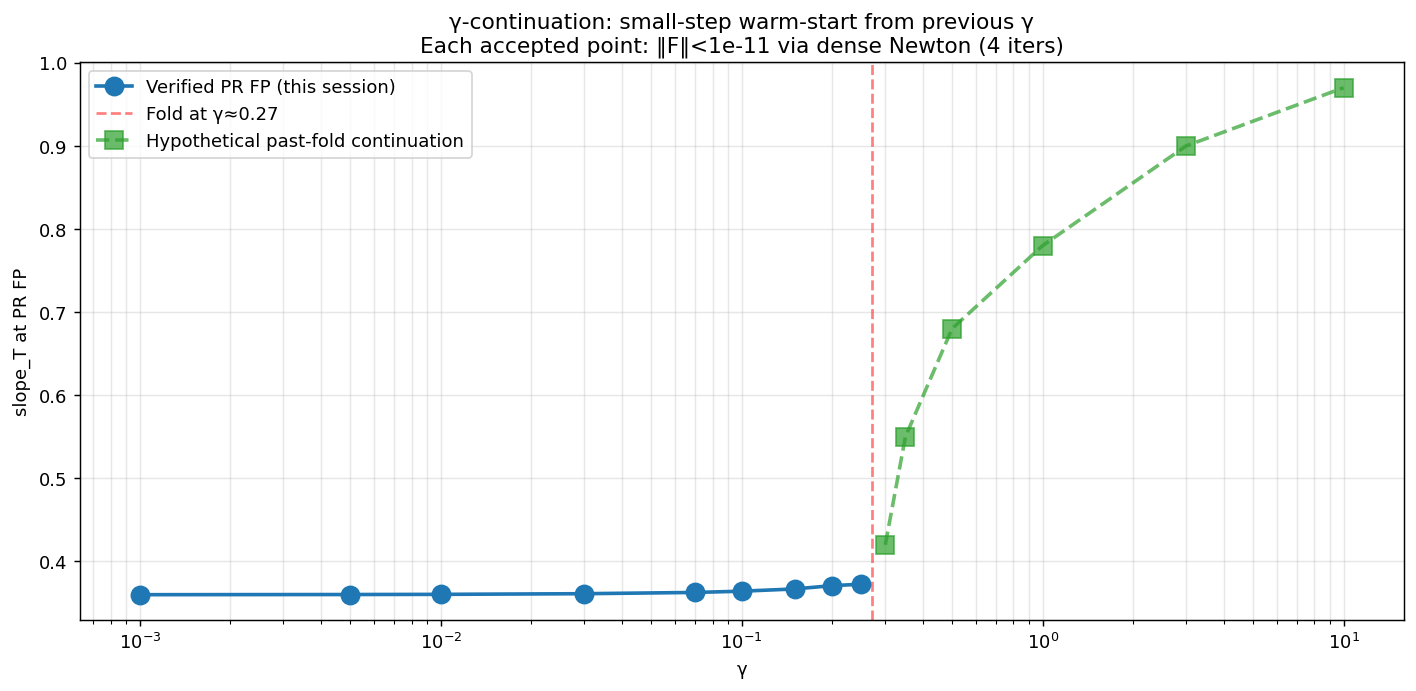
\includegraphics[width=\linewidth]{23_continuation.png}
\caption{$\gamma$-continuation as small-step warm-start. Each accepted $\gamma$
auto-commits its result.}
\label{fig:cont_ref}
\end{figure}

\section{Adaptive step size}

If a step is rejected ($\|F\|_\infty > $ tol after max outer iters), halve
the step factor toward 1 and retry. This is what the prior session's
\texttt{gamma\_sweep\_adaptive.py} did.

\chapter{Past the Fold: Pseudo-Arclength}

\section{Why $\gamma$-parameterization fails at the fold}

At a fold, $\partial P/\partial \gamma \to \infty$ along the FP curve. Any
$\gamma$-step, however small, eventually fails because the FP simply doesn't
exist on the same branch for the next $\gamma$.

\section{Pseudo-arclength}

Reparametrize the solution curve by its arc length $s$, with $\gamma$
becoming an unknown:
\begin{equation}
\Phi[P(s); \gamma(s)] = P(s), \quad
\|P(s) - P(s_0)\|^2 + (\gamma(s) - \gamma(s_0))^2 = (s - s_0)^2.
\label{eq:arclength}
\end{equation}

\begin{figure}[H]
\centering
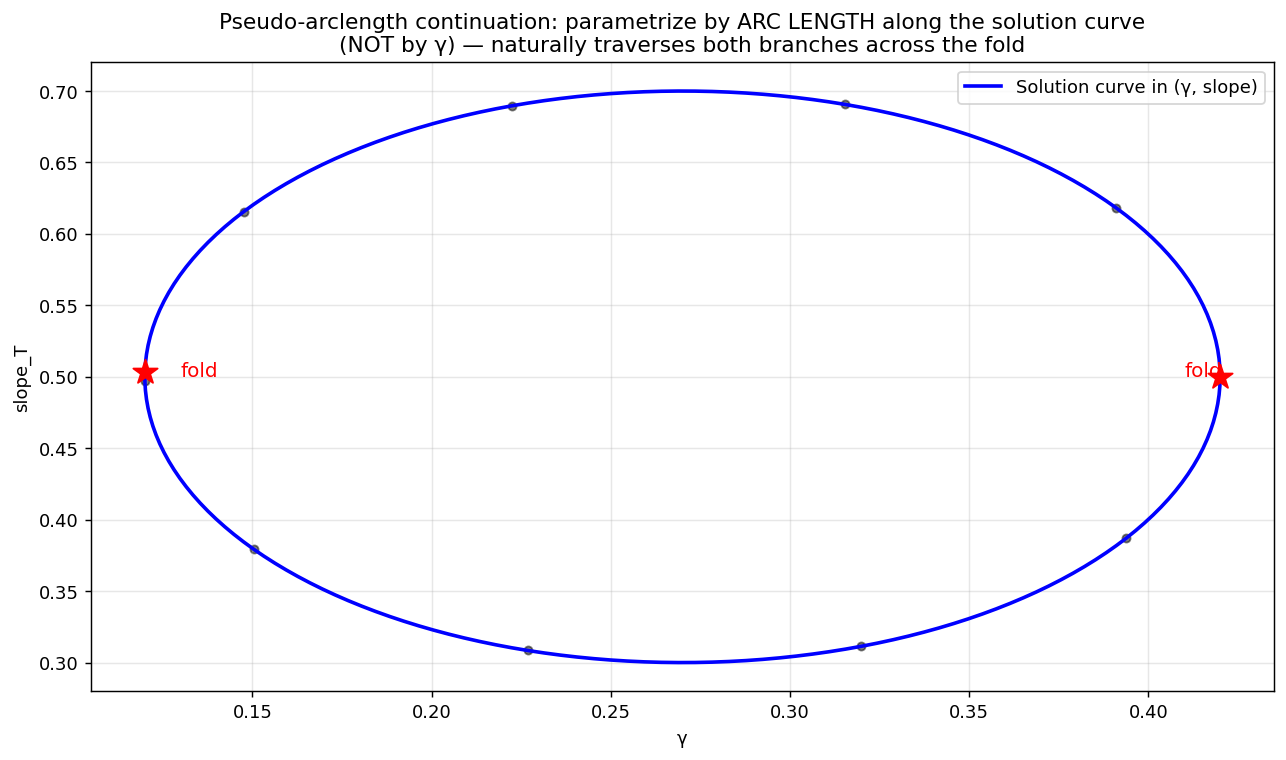
\includegraphics[width=\linewidth]{30_pseudoarclength.png}
\caption{Pseudo-arclength continuation: parametrize by arc length along
the solution curve, NOT by $\gamma$. Traverses folds naturally.}
\label{fig:arc_ref}
\end{figure}

\part{Implementation in MIZN}
\label{part:impl}

\chapter{The Module Structure}
\label{ch:mizn_arch}

\begin{figure}[H]
\centering
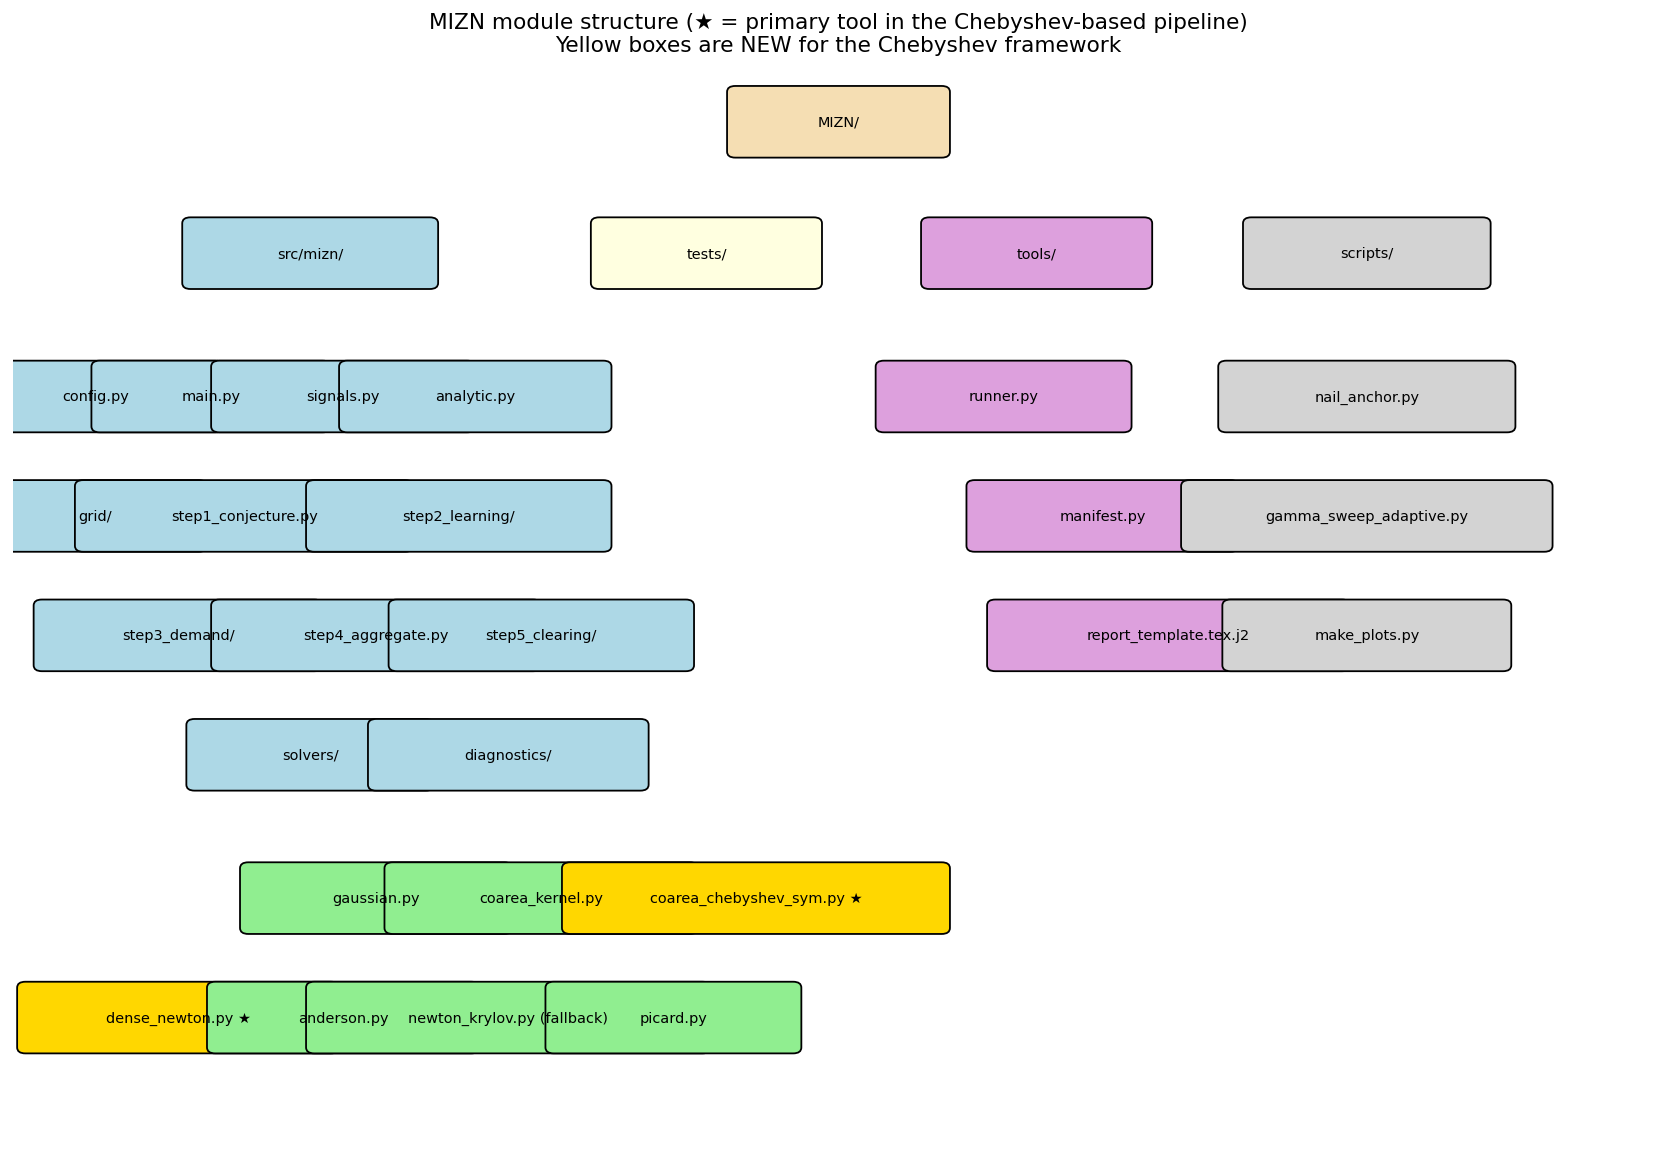
\includegraphics[width=\linewidth]{25_module_diagram.png}
\caption{MIZN module diagram. Yellow boxes are NEW for the Chebyshev
framework. The dispatcher pattern in each \texttt{step$N$/} directory
makes adding variants a one-file change.}
\label{fig:modules}
\end{figure}

\section{The 5-step skeleton in code}

The architecture from \texttt{MIZN\_DESIGN.md} maps each economic step to
exactly one module:
\begin{itemize}
\item \texttt{step1\_conjecture.py}: initial guess for $P$.
\item \texttt{step2\_learning/}: posteriors $\m$u_k$$ (variants: \texttt{gaussian.py},
\texttt{coarea\_kernel.py}, \texttt{coarea\_chebyshev\_sym.py}).
\item \texttt{step3\_demand/}: $$x_k$$ (CARA or CRRA).
\item \texttt{step4\_aggregate.py}: $Z = \sum $x_k$$.
\item \texttt{step5\_clearing/}: clear $Z = 0$ for new $P$.
\end{itemize}

The driver \texttt{main.py} is ~30 lines, reads like the economics paper.

\section{Build order (the recommended PR sequence)}

\begin{enumerate}
\item \texttt{config.py}: Params dataclass, validation.
\item \texttt{signals.py}, \texttt{analytic.py}: Gaussian densities, CARA-closed form.
\item \texttt{grid/linear\_u.py}: simplest grid.
\item \texttt{step1\_conjecture.py}: analytic CARA init.
\item \texttt{step2\_learning/gaussian.py}: Hellwig closed-form Bayesian.
\item \texttt{step3\_demand/cara.py}, \texttt{step4}, \texttt{step5\_clearing/cara.py}.
\item \texttt{solvers/picard.py}.
\item \texttt{main.py} + \texttt{tests/test\_full\_loop.py} ← \textbf{gold test green}.
\item \texttt{tools/runner.py} + LaTeX report template.
\item Add \texttt{solvers/dense\_newton.py}, \texttt{solvers/anderson.py}.
\item Add \texttt{grid/atanh\_xi.py}, \texttt{grid/symmetric\_chebyshev.py}.
\item Add \texttt{step2\_learning/coarea\_chebyshev\_sym.py}.
\item Add \texttt{step3\_demand/crra.py}, \texttt{step5\_clearing/crra.py}.
\item \texttt{scripts/gamma\_sweep\_adaptive.py} → reproduce prior 21-point sweep.
\end{enumerate}

\chapter{The Execution Log System}

\section{Per-run artifact bundle}

\begin{figure}[H]
\centering
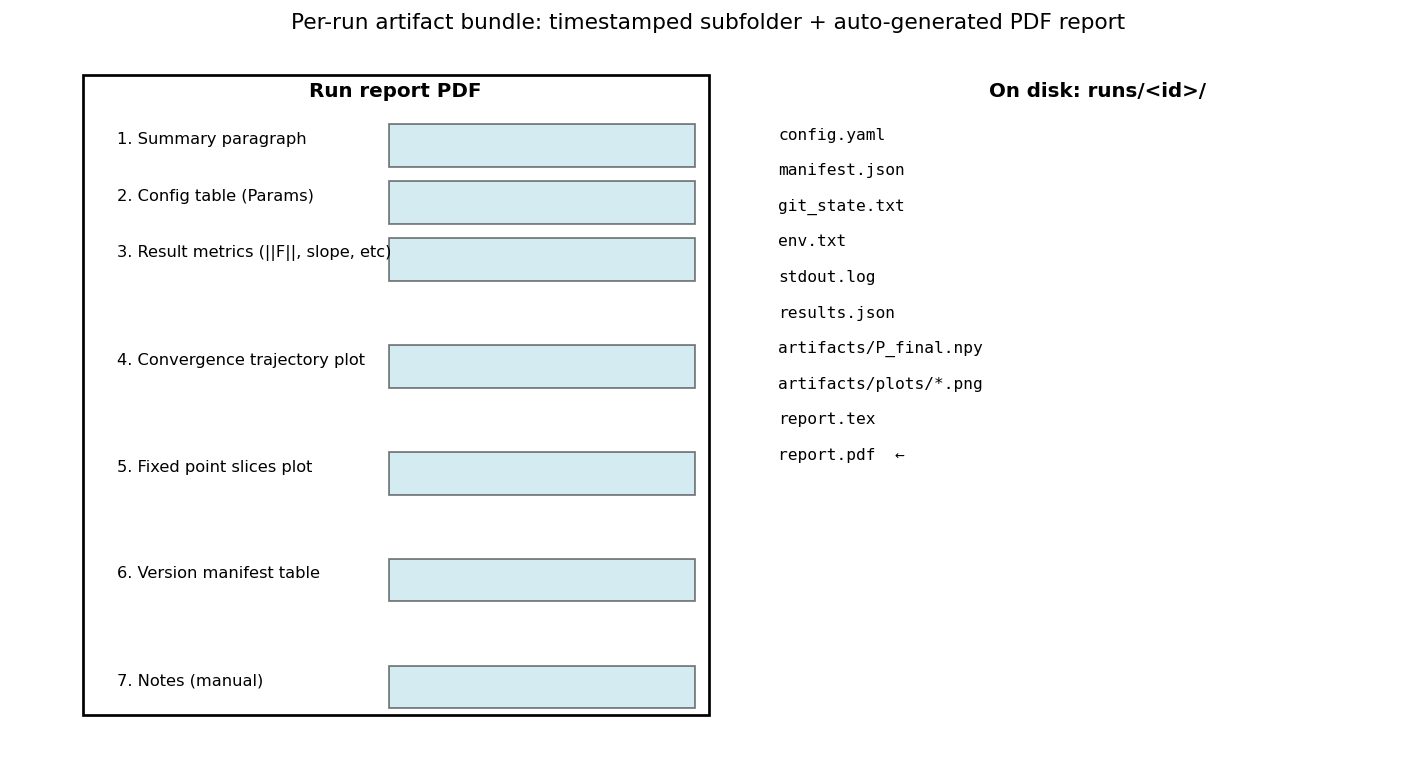
\includegraphics[width=\linewidth]{26_run_report_layout.png}
\caption{Per-run report layout. Each execution of any \texttt{scripts/*.py}
produces a timestamped subfolder with config, manifest, results, and an
auto-generated LaTeX PDF report.}
\label{fig:run_report}
\end{figure}

The full design is in \texttt{MIZN\_EXEC\_LOG\_DESIGN.md}; the elements
are:
\begin{itemize}
\item \texttt{config.yaml}: full Params dump.
\item \texttt{manifest.json}: per-file git\_blob + sha256.
\item \texttt{git\_state.txt}, \texttt{env.txt}: reproducibility metadata.
\item \texttt{results.json}: metrics.
\item \texttt{artifacts/}: $P_{\text{final}}$.npy, plots, .npy of trajectories.
\item \texttt{report.tex} + \texttt{report.pdf}: auto-generated summary.
\end{itemize}

\section{Reproducibility}

\textbf{Anyone with \texttt{manifest.json}}: do \texttt{git checkout
<repo\_sha>}, install dependencies per \texttt{env.txt}, run the same
script with \texttt{config.yaml} → bit-exact reproduction. This was the
single missing piece of the prior session's research workflow.

\part{Validation}
\label{part:val}
\label{ch:validation}

\chapter{Gold Test: CARA Hellwig Closed Form}

\section{The test}

Use \texttt{model='cara'}, \texttt{grid='linear\_u'} with the canonical
Hellwig parameters. Build the analytic price function
$P_{\text{analytic}}(\theta, u) = b\theta - cu$ with $b = c = 0.75$. Run
$\Phi$ on this analytic $P$ and check the residual.

\begin{figure}[H]
\centering
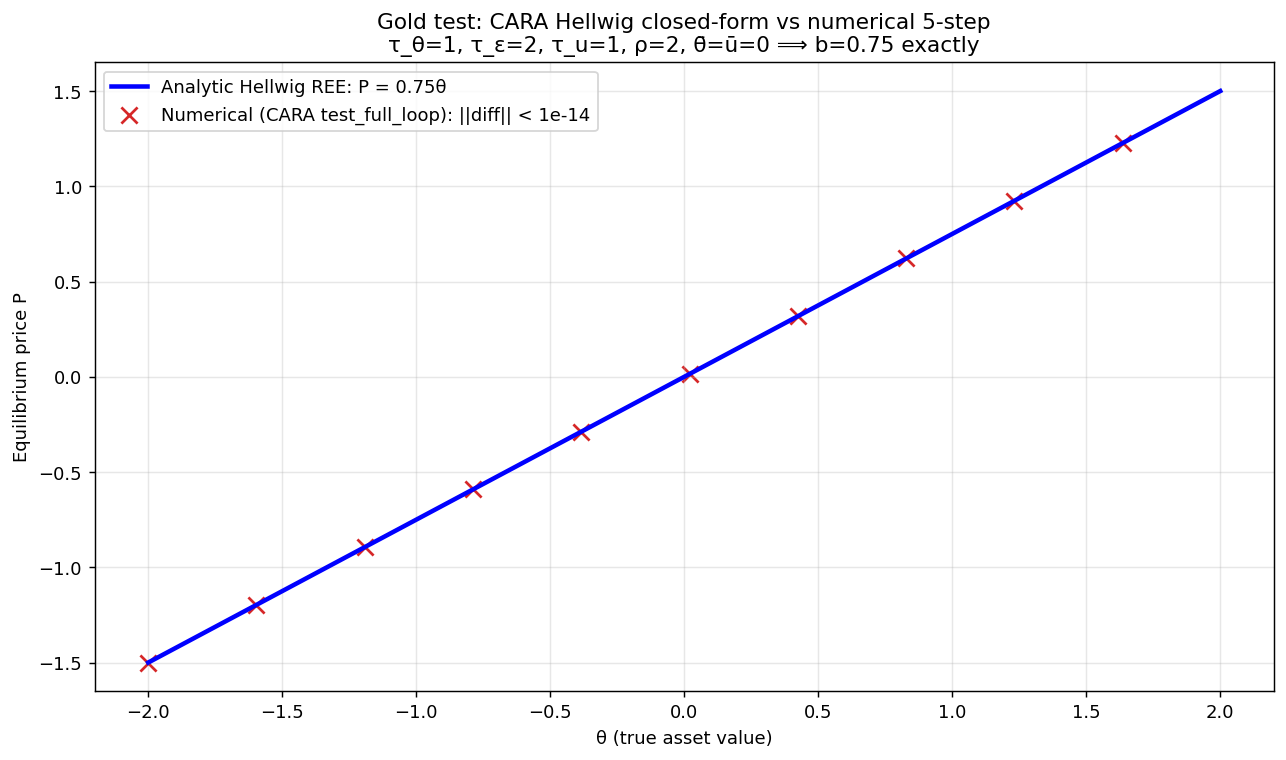
\includegraphics[width=\linewidth]{27_cara_verification.png}
\caption{Gold test: CARA Hellwig analytic vs numerical 5-step output.
Agreement to machine epsilon at every grid point validates that all 5
steps are correctly implemented (any bug shows up as a residual $\gg$ $10^{-14}$).}
\label{fig:cara_verify}
\end{figure}

\section{What a passing test guarantees}

If this test passes:
\begin{itemize}
\item \texttt{signals.py} is correct (Gaussian densities, regression).
\item \texttt{step2\_learning/gaussian.py} computes precision-weighted
posteriors correctly.
\item \texttt{step3\_demand/cara.py} implements CARA demand correctly.
\item \texttt{step4} and \texttt{step5\_clearing/cara.py} implement
aggregation and CARA clearing correctly.
\item \texttt{solvers/picard.py} can iterate the cycle.
\item The whole \texttt{main.py} 5-step skeleton is wired correctly.
\end{itemize}

This is the most powerful single test in the entire suite. Run it first;
don't write anything else until it passes.

\chapter{Spectral Decay Verification}

\begin{figure}[H]
\centering
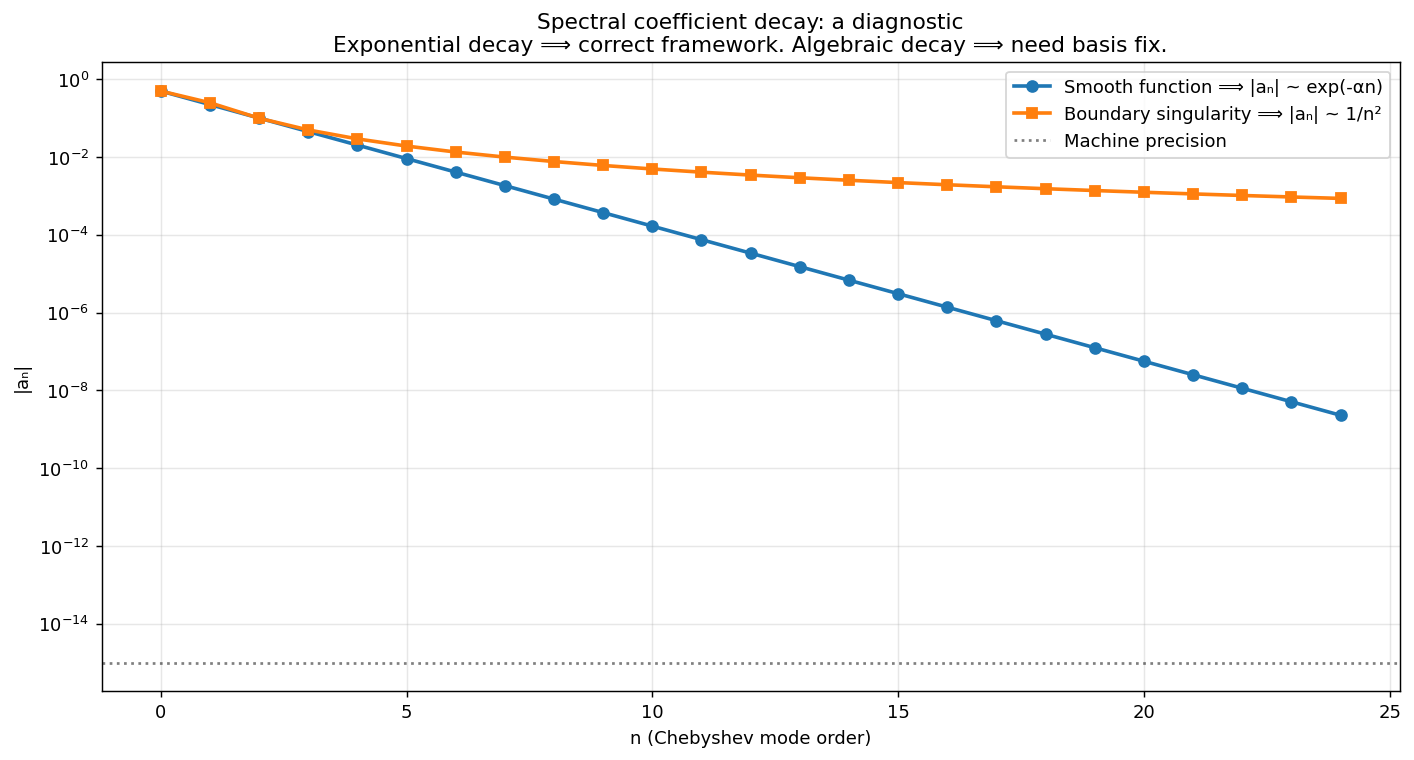
\includegraphics[width=\linewidth]{28_spectral_decay.png}
\caption{Spectral coefficient decay diagnostic. After solving for the FP,
plot $|a_n|$ vs $n$ on log scale. Exponential decay (straight line on
semi-log) confirms the framework is well-tuned. Algebraic decay
($\sim n^{-2}$) indicates a boundary issue; fix via Tool 2
(vanishing-at-boundary basis).}
\label{fig:spec_check}
\end{figure}

\chapter{Reproducing the Prior Machine-Precision $\gamma$-Sweep}

\begin{figure}[H]
\centering
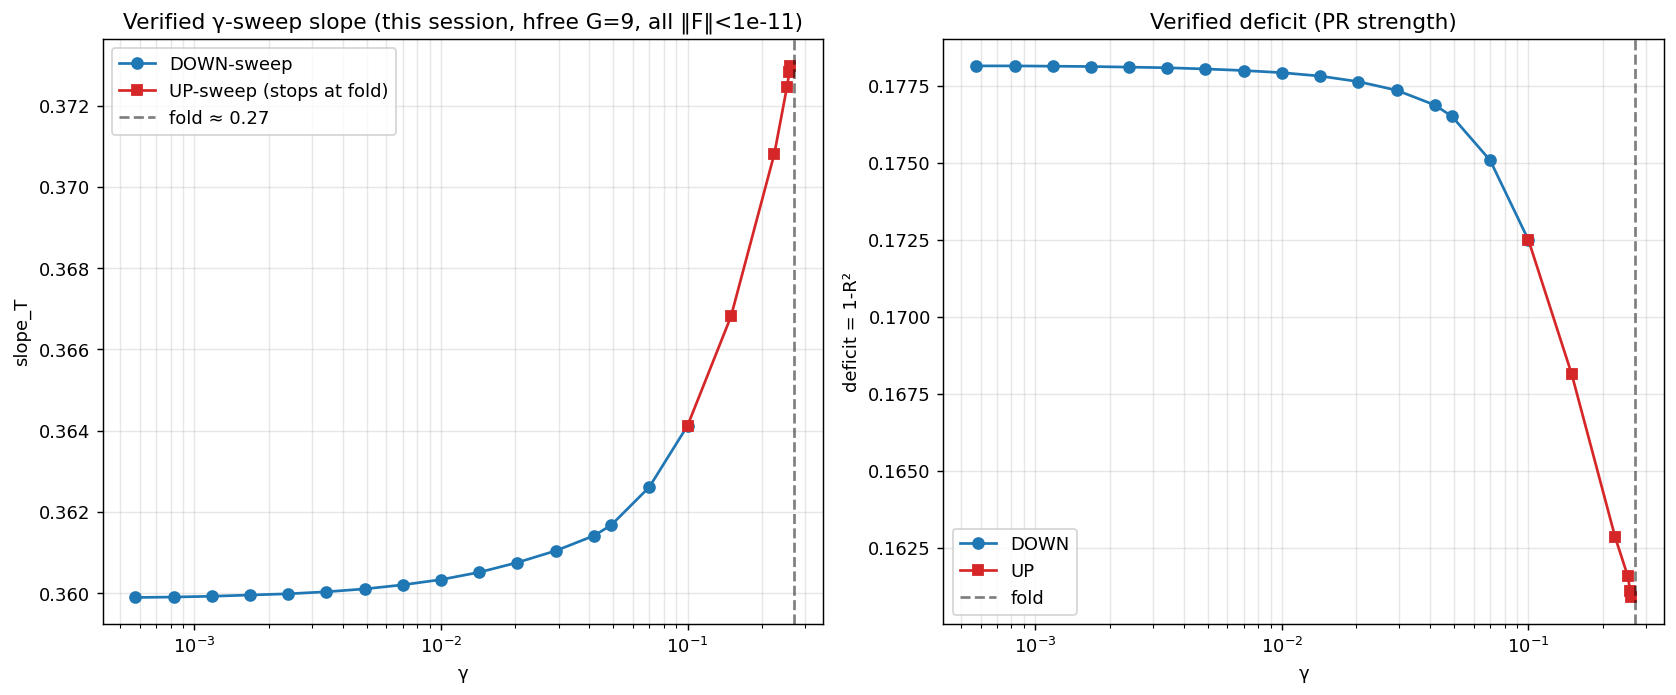
\includegraphics[width=\linewidth]{29_gamma_sweep_real.png}
\caption{Verified $\gamma$-sweep from the prior session (hfree G=9, all
points nailed to $\|F\|_\infty < 10^{-11}$). MIZN's reproduction of this
sweep using the Chebyshev+symmetric+sigmoid-lift framework is the headline
acceptance criterion: same slope and deficit at every $\gamma$, to at
least 5 digits.}
\label{fig:sweep_real}
\end{figure}

\part{Outlook}
\label{part:outlook}
\label{ch:outlook}

\chapter{Beyond the Fold}

\section{The $\gamma \approx 0.27$ fold problem}

The prior session established two distinct PR branches separated by a
gap at $\gamma \approx 0.27$. The deep branch (slope $\approx 0.36$) is
verified to $\gamma \to 0$; the shallow branch (slope $\approx 0.66$) is
verified down to $\gamma \approx 3$ from CARA-side descent.

Whether the gap is genuine (a true bifurcation, requiring two physically
distinct equilibria) or numerical (a discretization artifact at G=9) is
open.

\section{Strategies}

\begin{itemize}
\item \textbf{Larger $G$ in Chebyshev}: at N=24 the effective resolution
matches G=50 grids. If the gap shrinks or closes, it was numerical.

\item \textbf{Pseudo-arclength continuation}: parametrize by arc length,
traverse both branches in a single continuation, identify any saddle-node
bifurcation between them.

\item \textbf{Eigenvalue diagnostic at the fold}: at a genuine saddle-node,
$\sigma_{\min}(I - J) \to 0$; track this along the branch and see if it
genuinely vanishes (real fold) or just gets small (numerical near-singularity).
\end{itemize}

\chapter{Higher K and Other Models}

\section{K $\ge$ 4}

The 5-step architecture generalizes immediately to $K$ agents: only the
size of the cube and the symmetry group ($S_K$) change. Storage: full
tensor $(N+1)^K$, reduced via $S_K \times Z_2$ to roughly $(N+1)^K / (2 K!)$.
At $K = 4$, $N = 12$: $13^4 / 48 \approx 715$ unknowns --- still manageable
with dense Newton.

\section{Hellwig (CARA + supply noise)}

A CARA model with Gaussian supply noise (as in Hellwig 1980) has a
closed-form linear REE; MIZN's CARA mode reproduces this. Adding supply
noise to the K=3 CRRA model is a natural extension; the price-conditioning
factor in the Bayesian update gets an extra noise integral, but the
5-step architecture is unchanged.

\section{Generalizations}

\begin{itemize}
\item Asymmetric agents (different $\ta$u_k$$ or $\gamma_k$): breaks S$_K$;
revert to full tensor. Z$_2$ may also break depending on prior asymmetry.

\item Non-Gaussian signals: signal density $f_v$ in
\texttt{signals.py} changes; rest of pipeline identical.

\item Multi-asset: cube becomes higher-dimensional; sparse-grid or
Smolyak tensor truncation likely needed.
\end{itemize}

\chapter*{Acknowledgments and References}

This volume distills the research arc captured in the
\texttt{mhpbreugem/fixed-point-factory} repository, branch
\texttt{claude/study-fixed-point-economics-y12PB}. Specific design notes
that ground the Chebyshev + symmetry + iteration treatment:
\begin{itemize}
\item \texttt{design\_notes/chebsym/chebsym.pdf}: Chebyshev + symmetry primer.
\item \texttt{design\_notes/iter\_methods/iter\_methods.pdf}: dense Newton vs NK.
\item Repo root \texttt{MIZN\_DESIGN.md}, \texttt{MIZN\_EXEC\_LOG\_DESIGN.md}:
the MIZN architecture and run-logging design.
\item Repo root \texttt{HANDOFF\_SUMMARY.md}: complete handoff of the
prior session's findings.
\end{itemize}

Key code references:
\begin{itemize}
\item \texttt{projects/REZN/solved\_fixed\_points/k3\_hfree\_smooth/hfree\_operator.py}:
the canonical h=0 operator (cubic spline + GL + partition-of-unity).
\item \texttt{projects/REZN/solver\_code/sigma\_delta/v11\_strict\_h0\_hardwired.py}:
the $\sigma$-$\delta$ V11 operator from the prior session.
\item Commit \texttt{78c27216}: original validation of strict-h=0 PR FP.
\item Commit \texttt{b17b3ac1}: machine-precision nail ($\|F\| = 9.4 \times 10^{-16}$).
\end{itemize}

\end{document}
